\documentclass[titlepage=true, parskip=full]{scrartcl}
\usepackage[utf8]{inputenc} % use utf8 file encoding for TeX sources
\usepackage[T1]{fontenc}    % avoid garbled Unicode text in pdf
\usepackage{palatino}	      % because "Computer Modern" standard font is illegible
\usepackage{mathpazo}
\usepackage{amsmath}
\usepackage[ngerman]{babel}  % german hyphenation, quotes, etc
\usepackage{hyperref}       % detailed hyperlink/pdf configuration
\hypersetup{                % ‘texdoc hyperref‘ for options
	pdftitle={PSE: Entwurfsdokumentation},%
	bookmarks=true,%
}
\usepackage{graphicx}       % provides commands for including figures
\usepackage{csquotes}       % provides \enquote{} macro for "quotes"
\usepackage[nonumberlist, numberedsection]{glossaries}     % provides glossary commands
\usepackage{enumitem}
\usepackage{tikz}
\usepackage{tikz-uml}
\usepackage{tikz-er2}
\usepackage{comment}
\usepackage{array}
\usepackage{longtable}
\usepackage{hhline}
\usepackage{placeins}
\usepackage{needspace}
\usepackage[toc, page]{appendix}
\usepackage{tabularx}
\usepackage{tabulary}
\usepackage{multirow}
\usepackage{multicol}

\usepackage{microtype}
\usepackage{MnSymbol}
\usetikzlibrary{positioning}
\usepackage{pgfgantt}
\usepackage{float}
\usepackage{listings}
\usepackage{xcolor}

\colorlet{punct}{red!60!black}
\definecolor{background}{HTML}{EEEEEE}
\definecolor{delim}{RGB}{20,105,176}
\colorlet{numb}{magenta!60!black}

% Kommandos für Atomare und JSON-Werte:
\newcommand{\jsonatom}[1]{$\langle\textnormal{\textit{#1}}\rangle$}
\newcommand{\jsonobj}[1]{$\llangle\textnormal{\textit{#1}}\rrangle$}
\newcommand{\jsonpart}[2]{$\llangle\textnormal{\textit{#1}\,[#2]}\rrangle$}

\lstdefinelanguage{json}{
    basicstyle=\normalfont\ttfamily,
    numbers=left,
    numberstyle=\scriptsize,
    escapeinside={(*}{*)},
    stepnumber=1,
    numbersep=8pt,
    showstringspaces=false,
    breaklines=true,
    frame=lines,
    backgroundcolor=\color{background},
    literate=
     *{0}{{{\color{numb}0}}}{1}
      {1}{{{\color{numb}1}}}{1}
      {2}{{{\color{numb}2}}}{1}
      {3}{{{\color{numb}3}}}{1}
      {4}{{{\color{numb}4}}}{1}
      {5}{{{\color{numb}5}}}{1}
      {6}{{{\color{numb}6}}}{1}
      {7}{{{\color{numb}7}}}{1}
      {8}{{{\color{numb}8}}}{1}
      {9}{{{\color{numb}9}}}{1}
      {:}{{{\color{punct}{:}}}}{1}
      {,}{{{\color{punct}{,}}}}{1}
      {\{}{{{\color{delim}{\{}}}}{1}
      {\}}{{{\color{delim}{\}}}}}{1}
      {[}{{{\color{delim}{[}}}}{1}
      {]}{{{\color{delim}{]}}}}{1},
}


\usepackage[vlined]{algorithm2e}
% see http://ctan.math.utah.edu/ctan/tex-archive/macros/latex/contrib/algorithm2e/doc/algorithm2e.pdf  for more information
\DontPrintSemicolon
\SetKwSwitch{Switch}{Case}{Other}{case}{of}{}{else}{}{}
\SetKw{KwAssert}{assert}
\SetKw{KwInvariant}{invariant}
\SetKw{KwStep}{step}
\SetKw{KwDownto}{downto}	
\SetKw{KwArrayOf}{array of }
\SetKw{KwArray}{array }
\SetKw{KwOf}{ of }
\SetKw{KwNot}{ not }
\SetKw{KwIs}{ is }
\SetKw{KwAnd}{ and }
\SetKw{KwOr}{ or }
\SetKw{KwBreak}{break}
\SetKw{KwThrow}{throw}
\SetKw{KwTrue}{true}
\SetKw{KwFalse}{false}
\SetKwBlock{KwFunc}{function}{}
\SetKwBlock{KwProc}{procedure}{}
\newcommand{\Function}[2]{\KwFunc({#1}){#2}}
\newcommand{\Procedure}[2]{\KwProc({#1}){#2}}
\SetKwData{KwList}{List}
\SetKwData{KwSet}{Set}
\newcommand{\KwListOf}{\KwList \KwOf}
\newcommand{\KwSetOf}{\KwSet \KwOf}
\SetKwComment{Comment}{// }{}
\newcommand{\LComment}[1]{\hspace{-2pt}\Comment*[l]{#1}}
\newcommand{\RComment}[1]{$ \qquad $ \Comment*[h]{#1} \\}
\newcommand{\RCommentNoBreak}[1]{$ \qquad $ \Comment*[h]{#1}}
\newcommand{\MyCommentSty}[1]{\emph{\textcolor{gray}{#1}}}
\SetCommentSty{MyCommentSty}
\SetFuncSty{emph}
\definecolor{kwblue}{rgb}{0.3,0.3,1}
\newcommand{\MyKwSty}[1]{\textcolor{kwblue}{\textbf{#1}}}
\SetKwSty{MyKwSty}
\newcommand{\Call}[2]{\FuncSty{#1}(#2)}
\newcommand{\pluseq}{\mathrel{+}=}
\newcommand{\Var}[1]{\textit{#1}}

% needed to define linebreak points without hyphenation (useful for URL wrapping)
\newcommand{\+}{\discretionary{}{}{}}

\renewcommand{\arraystretch}{1.24}  % for proper row spacing in tables

%%%%%%%%%%%%%%%%%%%%%%%%%%%
% longtable multirow page break insanity fix – http://tex.stackexchange.com/a/52101
\makeatletter
\def\@cline#1-#2\@nil{%
	\omit
	\@multicnt#1%
	\advance\@multispan\m@ne
	\ifnum\@multicnt=\@ne\@firstofone{&\omit}\fi
	\@multicnt#2%
	\advance\@multicnt-#1%
	\advance\@multispan\@ne
	\leaders\hrule\@height\arrayrulewidth\hfill
	\cr
	\noalign{\nobreak\vskip-\arrayrulewidth}}
\makeatother
%%%%%%%%%%%%%%%%%%%%%%%%%%%

% For Christ's sake, I'm sick and tired of this f*cking orphan/widow crap!
\widowpenalty=10000
\clubpenalty=10000
% Source: somewhere on tex.stackexchange.com

\renewcommand{\to}{\longrightarrow} % proper math typography
\newcommand{\NN}{\mathbb{N}}
\newcommand{\RR}{\mathbb{R}}
\newcommand{\QQ}{\mathbb{Q}}

\addto\captionsngerman{\let\appendixtocname\appendixname\let\appendixpagename\appendixname}

% fix hyphenation
\hyphenation{Log-out Log-in Ak-tions Ak-tion ge-öff-net liken dis-liken Like Dis-like No-ti-fi-ca-tion Mo-dule inkl Au-tho-ri-za-tion Web-App}

\usepackage{enumitem}
\setlist[itemize]{nosep}
\shorthandon{"}
\makeglossaries
%
% % Automatisch generiertes Glossar
%
%\glsaddall % das sorgt dafür, dass alles Glossareinträge gedruckt werden, nicht nur die verwendeten. Das sollte nicht nötig sein!
%
% % Glossareinträge
%
\newglossaryentry{Rest}
{
	name=REST,
	description={Abk. für Representational State Transfer, Programmierparadigma für \glspl{Webservice} auf Basis des HTTP-Protokolls}
}

\newglossaryentry{ECTS-Punkte}
{
	name=ECTS-Punkte,
	description={Leistungspunkte, die für ein erfolgreich absolviertes \gls{Modul} von der Hochschule auf Basis des ECTS-Punktesystems vergibt werden, und mit denen der Arbeitsaufwand gemessen wird},
}

\newglossaryentry{Generierungs-Tool}
{
	name=Generierungs-Tool,
	description={Tool, für die automatische Erstellung bzw. Vervollständigung von Studienpläne},
}


\newglossaryentry{Webservice}
{
	name=Webservice,
	plural=Webservices,
	description={Softwareanwendung, die über ein Netzwerk bereitgestellt wird}
}

\newglossaryentry{Plug-In-Paket}
{
	name=Plug-In-Paket,
	plural=Plug-In-Pakete,
	description={Paket bestehend aus mehreren \glspl{Plug-In}}
}

\newglossaryentry{iMage}
{
	name={iMage},
	description={Bildbearbeitungssoftware der Firma SWT. Bietet im Basispaket nur Funktionalitäten zur Skalierung und Drehung von Bildern}
}

\newglossaryentry{Internetbrowser}
{
	name={Internetbrowser},
	description={Programm, mit dem Websites gefunden, gelesen und verwaltet werden können, mit aktiviertem JavaScript}
}

\newglossaryentry{Online-Shop}
{
	name={Online-Shop},
	description={Internetseite, die Produkte zum Kauf anbietet}
}

\newglossaryentry{KIT}
{
	name=KIT,
	description={Das Karlsruher Institut für Technologie ist die Forschungsuniversität in der Helmholtz-Gemeinschaft. Standort der Universität ist Karlsruhe. }
}

\newglossaryentry{SCC}
{
	name=SCC,
	plural=SCC,
	description={Das Steinbuch Center for Computing ist ein Institut und das zentrale Rechenzentrum des \gls{KIT}s.}
}

\newglossaryentry{Benutzer}
{
	name=Benutzer,
	plural=Benutzer,
	description={Ein am \gls{KIT} eingeschriebener Student, der über ein gültigen Account beim \gls{SCC} verfügt.}
}

\newglossaryentry{Wizard}
{
	name=Wizard,
	plural=Wizards,
	description={Ein Wizard ist ein Subsystem, welches einen \gls{Benutzer} visuell durch eine Systemfunktionalität führt und dabei vom \gls{Benutzer} bestimmte Interaktionen mit dem System fordert.}
}

\newglossaryentry{Drag-and-Drop}
{
	name=Drag-and-Drop,
	description={(deutsch: "Ziehen und Ablegen") Eine Methode zur Bedienung grafischer Benutzeroberflächen bei der grafische Elemente mittels eines Mauszeigers bewegt werden.}
}

\newglossaryentry{Shibboleth Identity Provider}
{
	name=Shibboleth Identity Provider,
	description={Ein genau spezifiziertes System zum Login mittels einer von einer dritten Instanz bereitgestellten Identität.}
}

\newglossaryentry{Studiengang}
{
	name=Studiengang,
	description={Ein vom KIT angebotener, auf einer Studien- und Prüfungsordnung und einem Modulhandbuch basierender Studiengang.}
}

\newglossaryentry{Semester des Studienbeginns}
{
	name=Semester des Studienbeginns,
	description={Das Semester in welchem der \gls{Benutzer} im ersten Fachsemester des \gls{Studiengang}s war.}
}

\newglossaryentry{Modul}
{
	name=Modul,
	plural=Module,
	description={Ein Modul ist ein Teilblock des Studiums, welcher aus verschiedenartigen Veranstaltungen (genannt \glspl{Teilmodul}) bestehen kann und für welchen man nach Ablegung eventueller \glspl{Modulpruefung} eine festgelegte Anzahl an ECTS-Punkten erhält.}
}
\newglossaryentry{Teilmodul}
{
	name=Teilmodul,
	plural=Teilmodule,
	description={Ein Teilmodul ist eine universitäre Veranstaltung, welche als Teil eines Moduls besucht werden kann und mittels einer (wie auch immer gearteten) \gls{Modulpruefung} bestanden werden kann.}
}
\newglossaryentry{Modulpruefung}
{
	name=Modulprüfung,
	plural=Modulprüfungen,
	description={Eine Modulprüfung ist eine Prüfung, welche abgelegt werden muss um ein Modul \glslink{Modul abgeschlossen}{abzuschließen}.}
}
\newglossaryentry{Zur Pruefung angetreten}
{
	name=Zur Pruefung angetreten,
	description={Ein \gls{Benutzer} ist zu einer \gls{Modulpruefung} angetreten, wenn er sich fristgerecht für selbige angemeldet und nicht fristgerecht abgemeldet hat.}
}

\newglossaryentry{Modul abgeschlossen}
{
	name=Modul abgeschlossen,
	description={Ein \gls{Modul} gilt als abgeschlossen, wenn der \gls{Benutzer} alle nach Modulhandbuch notwendigen \glspl{Modulpruefung} bestanden hat.}
}

\newglossaryentry{Modul begonnen}
{
	name=Modul begonnen,
	description={Ein \gls{Modul} gilt als begonnen, wenn der \gls{Benutzer} zu mindestens einer \gls{Modulpruefung} \glslink{Zur Pruefung angetreten}{angetreten} ist.}
}

\newglossaryentry{Studienplan}
{
	name=Studienplan,
	plural=Studienpläne,
	description={Eine Zusammenstellung von Modulen, in welcher enthalten ist wann welches Modul planmäßig \glslink{Modul begonnen}{begonnen} werden soll.}
}
\shorthandoff{"}

\begin{document}
	
\begin{titlepage}
	\centering
	{\huge \bfseries \sffamily Studienplanung als Generierung von Workflows mit Compliance-Anforderungen: Planerstellung und Visualisierung\par}
	\vspace{1cm}
	{\LARGE Entwurfsdokumentation\par}
	\vfill
	\begin{tabular}{>{\Large}c}
		Nada Chatti\\
		Daniel Jungkind\\
		\textbf{Hannes Kuchelmeister}\\
		Ulrike Rheinheimer\\
		Paul Samuel M. Teuber\\
		Tim Niklas Uhl
	\end{tabular}
	\vfill
	11. Januar 2017
\end{titlepage}
\tableofcontents
\pagebreak

%
% % Hier beginnt die Gliederung des Pflichtenhefts
\section{Einleitung}
Der Implementierungsbericht des Projekts „Studienplanung als Generierung von Workflows mit Compliance-Anforderungen: Planerstellung und Visualisierung“ beschreibt die Umsetzung des zuvor im Pflichtenheft und Entwurf spezifizierten Projekts. In über ????? Zeilen Java-, Javascript-, HTML- und CSS-Code liegt jetzt eine fertige, nur noch zu optimierende Anwendung vor. In diesem Bericht möchten wir dabei auf implementierte und ausgelassen Features eingehen, Änderungen beschreiben und begründen, und die Implementierungsphase (einschließlich aller durchgemachten Nächte) reflektieren.
Zusammenfassend ist dieser Bericht Ende einer arbeitsintensiven, aber erfolreichen Phase, die als Endprojekt ein einmalig sinnvolles, dringendnotweniges und jedem Studenten zu empfehlendes Studienplanungshilfsmittel zur Verfügung stellt.



 
\section{Aufbau}

\subsection{Architektur}

\subsubsection{Server}

\subsubsection{Client}
Der Client besteht aus einer leicht abgewandelten Model-View-Controller-Architektur (MVC-Architektur), die auf Backbone.js \cite{backbone} basiert.
Das System besteht aus 4 Haupt-Paketen: Storage, Model, View und Router.\\
Storage übernimmt die Kommunikation mit dem REST-Webservice sowie die Speicherung in Cookies. Somit bildet Storage die Zugriffsschicht für das Model-Paket. \\
Model bildet die Daten aus den Cookies und dem REST-Webservice auf Klassen ab und stellt Möglichkeiten zum Abruf sowie zur Speicherung zur Verfügung, die auf Storage basieren.\\
View zeigt die Daten aus dem Model an und aktualisiert im Fall einer Änderung des Models die Anzeige. Auch fängt das View-Paket Interaktionen mit der Benutzeroberfläche (wie Klicks oder Drag and Drop) ab und verarbeitet diese entsprechend.\\
Router übernimmt schließlich die Aufgaben des Controllers in klassischen MVC-Architekturen. Der Router wird bei Änderungen des URI Fragments aufgerufen und kann so beim Wechsel auf eine andere Seite der WebApp die neuen View-Klassen initialisieren und die zugehörigen Inhalte anzeigen.

\subsection{Klassendiagramm}  % necessary?

\section{REST-Webservice Spezifikation}
\subsection{Konvention}
Atomare Werte werden mittels \jsonatom{name} angegeben, wobei name ein eindeutiger Bezeichner für den Wert ist.\\
Zusammengesetzte JSON-Datenklassen werden mittels \jsonobj{name} angegeben, wobei name ein eindeutiger Bezeichner für das JSON-Datenklassen ist.\\
Teile einer zusammengesetzten JSON-Datenklasse werden mittels \jsonpart{name}{prop1, prop2, prop3} angegeben, wobei prop1, prop2, prop3 die einzigen Werte sind, welche angezeigt werden.
blub
\subsubsection{Module}
\begin{lstlisting}[language=json,firstnumber=1]
(*\jsonobj{Module}*) = {
	"id": (*\jsonatom{Modul-ID}*),
	"name": (*\jsonatom{Modul-Name}*),
	"category" : (*\jsonatom{Modul-Category-Name}*),
	"completed": (*\jsonatom{Modul-Completed}*)
	"semester": (*\jsonatom{Modul-Semester}*),
	"creditpoints": (*\jsonatom{Modul-Creditpoints}*),
	"lecturer": (*\jsonatom{Modul-Dozent}*),
	"preference" (*\jsonatom{Modul-Preferenz}*),
	"description": (*\jsonatom{Modul-Beschreibung}*),	
	"constrains": [(*\jsonobj{Constraint}*), ...]	
}
\end{lstlisting}

\subsubsection{Constraint}
\begin{lstlisting}[language=json,firstnumber=1]
(*\jsonobj{Constraint}*) = {
	"name": (*\jsonatom{Constraint-Name}*),
	"first": (*\jsonpart{Modul}{id}*),
	"second": (*\jsonpart{Modul}{id}*),
	"type": (*\jsonatom{Constraint-Typ}*),
	"descriptionFirst": (*\jsonatom{Constraint-Beschreibung}*)
	"descriptionSecond": (*\jsonatom{Constraint-Beschreibung}*)	
}
\end{lstlisting}

\subsubsection{Filter}
\begin{lstlisting}[language=json,firstnumber=1]
(*\jsonobj{Filter}*) = {
	"id": (*\jsonatom{Filter-ID}*),
	"name":(*\jsonatom{Filter-Name}*),
	"value": (*\jsonatom{Filter-Value}*),
	"tooltipp": (*\jsonatom{Filter-Tooltipp}*),
	"specification": (*\jsonobj{Filter-Eigenschaften}*)
}
\end{lstlisting}
\begin{lstlisting}[language=json,firstnumber=1]
(*\jsonobj{Filter-Eigenschaften}*) = {
	"type": (*\jsonatom{Filter-Typ}*),
	"value": (*\jsonatom{Filter-Value}*)

	EITHER (
		"max": (*\jsonatom{Filter-ID}*),
		"min": (*\jsonatom{Filter-Name}*),
	) OR (
		"items": [(*\jsonatom{Selectable-Item}*), ...]
	)
}
\end{lstlisting}

\subsubsection{Objective Function}
\begin{lstlisting}[language=json,firstnumber=1]
(*\jsonobj{Objective}*) = {
	"id": (*\jsonatom{Zielfunktion-ID}*),
	"name": (*\jsonatom{Zielfunktion-Name}*),
	"description": (*\jsonatom{Zielfunktion-Beschreibung}*)
}
\end{lstlisting}

\subsubsection{Studienplan}
\begin{lstlisting}[language=json,firstnumber=1]
(*\jsonobj{Studienplan}*) = {
	"id": (*\jsonatom{Studienplan-ID}*),
	"status": (*\jsonatom{Studienplan-Status}*),
	"creditpoints_sum":(*\jsonatom{Studienplan-Creditpoints-Sum}*),
	"name": (*\jsonatom{Studienplan-Name}*),
	"modules":[(*\jsonpart{Modul}{id, name, completed, semester, creditpoints, lecturer}*), ...]
	"violations": (*\jsonpart{Modul}{id, constrains}*)	
}
\end{lstlisting}

\subsubsection{CopyLink}
\begin{lstlisting}[language=json,firstnumber=1]
(*\jsonobj{CopyLink}*) = {
	"id": (*\jsonatom{Studienplan-ID}*),
	"token": (*\jsonatom{CopyToken}*)
}
\end{lstlisting}


\subsection{REST-Json}

\subsubsection{/plans}
POST:
\begin{lstlisting}[language=json,firstnumber=1]
{
	"plan": (*\jsonpart{Studienplan}{name}
}
\end{lstlisting}
POST return:
\begin{lstlisting}[language=json,firstnumber=1]
{
	"plan": (*\jsonpart{Studienplan}{name}
}
\end{lstlisting}
GET:
\begin{lstlisting}[language=json,firstnumber=1]
{
	"plans": [(*\jsonpart{Studienplan}{id, status, creditpoints-sum, name}*), ...]
}
\end{lstlisting}

\subsubsection{/plans/\{plan\_id\}}
GET, PUT
\begin{lstlisting}[language=json,firstnumber=1]
{
	"plan": (*\jsonpart{Studienplan}*)
}
\end{lstlisting}
PATCH
\begin{lstlisting}[language=json,firstnumber=1]
{
	"plan": (*\jsonpart{Studienplan}{name}*)
}
\end{lstlisting}
DELETE return
\begin{lstlisting}[language=json,firstnumber=1]
{
	"successful": <Delete-Success-Message>
}
\end{lstlisting}
POST
\begin{lstlisting}[language=json,firstnumber=1]
{
	"plan": (*\jsonpart{Studienplan}{name}*)
}
\end{lstlisting}
GET, PUT, POST, PATCH return
\begin{lstlisting}[language=json,firstnumber=1]
{
	"plan": (*\jsonpart{Studienplan}{id, status, creditpoints-sum, name}*)
}
\end{lstlisting}

\subsubsection{/plans/\{plan\_id\}/modules/}
Es sollten nur noch nicht abgeschlossene  Module zurückgegeben werden.\linebreak
GET (list of applied filters and their respective value as URL parameters):
\begin{lstlisting}[language=json,firstnumber=1]
{
	"modules":[(*\jsonpart{Modul}{id, name, creditpoints, lecturer, preference}*), ...]
}	
\end{lstlisting}

\subsubsection{/plans/\{plan\_id\}/modules/\{modul\_id\}}
GET:
\begin{lstlisting}[language=json,firstnumber=1]
{
	"module": (*\jsonobj{Modul}*)
}
\end{lstlisting}
PUT, PATCH:
\begin{lstlisting}[language=json,firstnumber=1]
{
	"module": (*\jsonpart{Modul}{id, semester}*)
}
\end{lstlisting}
DELETE
\begin{lstlisting}[language=json,firstnumber=1]
{
	"module": (*\jsonpart{Modul}{id}*)
}
\end{lstlisting}

\subsubsection{/plans/\{plan\_id\}/modules/\{modul\_id\}/preference}
PUT
\begin{lstlisting}[language=json,firstnumber=1]
{
	"module": (*\jsonpart{Modul}{id, preference}*)
}
\end{lstlisting}

\subsubsection{/plans/\{plan\_id\}/verification}
GET
\begin{lstlisting}[language=json,firstnumber=1]
{
	"plan": (*\jsonpart{Studienplan}{id,status, violations}*)
}
\end{lstlisting}

\subsubsection{/plans/\{plan\_id\}/proposal/\{objective\_id\}}
GET
\begin{lstlisting}[language=json,firstnumber=1]
{
	"plan": (*\jsonpart{Studienplan}{id, modules}*)
}
\end{lstlisting}

\subsubsection{/plans/\{plan\_id\}/pdf}
GET (just return pdf file)

\subsubsection{/plans/\{plan\_id\}/share}
GET
\begin{lstlisting}[language=json,firstnumber=1]
{
	"plan":(*\jsonobj{CopyLink}*)
}
\end{lstlisting}

\subsubsection{/filters}
GET
\begin{lstlisting}[language=json,firstnumber=1]
{
	"filters":[(*\jsonobj{Filter}*), ...]
}
\end{lstlisting}

\subsubsection{/objective-functions}
GET
\begin{lstlisting}[language=json,firstnumber=1]
{
	"functions":[(*\jsonobj{Objective}*), ...]
}
\end{lstlisting}
\subsection{Authentifizierung}
\label{subsec:api-auth}
\paragraph{Zugrundeliegende Spezifikation} Die Authentifizierung am REST-Webservice erfolgt über eine OAuth 2.0 Schnittstelle nach RFC 6749 (siehe \cite{rfc6749}).
Für das momentane System ist hierbei nur die Authentifizierung über \textit{Implicit-Grant} \cite[Kap. 4.2]{rfc6749} notwendig, jedoch sollte das System mindestens um \textit{Authorization-Code-Grant} \cite[Kap. 4.1]{rfc6749} und \textit{Resource-Owner-Password-Credentials-Grant} \cite[Kap. 4.3]{rfc6749} erweitert werden können, weshalb die Basis für diesen Authentifizierungstyp ebenfalls implementiert wird. Bei dem Versuch eine Authentifizierung mittels \textit{Authorization-Code-Grant} oder \textit{Resource-Owner-Password-Credentials-Grant} auszuführen, wird dann eine Fehlermeldung zurück gegeben.\\
Die zugrundeliegende Spezifikation verteilt klare Rollen an die verschiedenen Akteure, welche an der Interaktion der Systeme beteiligt sind. In Tabelle \ref{tab:api-auth-roles} ist angegeben, welches Subsystem die jeweiligen Rollen bei der OAuth-Authentifizierung in unserem System übernimmt

\begin{table}
	\begin{tabularx}{\textwidth}{@{} | X | X | @{}}
		\hline
		\textbf{Rolle} & \textbf{Subsystem}\\ \hline \hline
		\textit{resouce owner} & Benutzer \\ \hline
		\textit{resource server} & REST-Webservice \\ \hline
		\textit{client} & Aktuell ausschließlich die WebApp. Zukünftig vielleicht weitere Systeme, welche auf den REST-Webservice zugreifen \\ \hline
		\textit{authorization server} & REST-Webservice \\ \hline
		\textit{user agent} & Web-Browser des Benutzers \\
		\hline
	\end{tabularx}
	\caption{Rollen in der OAuth 2.0 Spezifikation}
	\label{tab:api-auth-roles}
\end{table}

\paragraph{Registrierung der Klienten}
Klienten sind bei der Authentifizierung alle auf den REST-Webservice zugreifenden Systeme, welche sich dafür im Namen eines Nutzers beim REST-Webservice authentifizieren.\\
Ein Beispiel für einen solchen Klienten ist die WebApp.\\
Alle Klienten werden in der Datenbank gespeichert.\\
Wir unterscheiden zwischen zwei Typen von Klienten: \textit{Vertrauenswürdige} sowie \textit{öffentliche} Klienten. Die Definitionen hierzu finden sich auch in \cite[Kap. 2.1]{rfc6749}. Bei der WebApp handelt es sich auf Grund der Zugänglichkeit des Codes und der Daten um einen öffentlichen Klienten.
\subparagraph{Vertrauenswürdiger Klient}
Für einen vertrauenswürdigen Klienten werden die Informationen aus Tabelle \ref{tab:api-auth-confidential-client-data} gespeichert.\\
\begin{table}
	\begin{tabularx}{\textwidth}{@{} | X | X | @{}}
		\hline
		\textbf{Name} & \textbf{Beschreibung}\\ \hline \hline
		\textit{api\_key} & Eindeutige, öffentliche ID des Klienten. Beginnt mit dem Präfix \enquote{key-} \\ \hline
		\textit{api\_secret} & Nur dem Klienten bekannte Kennung. Beginnt mit dem Präfix \enquote{secret-} \\ \hline
		\textit{scope} & Berechtigungen (auch mehrere) die der Klient anfordern darf. Vorerst immer nur \enquote{student} \\ \hline
		\textit{redirect\_url} & URL an welche beim \textit{Implicit-Grant} bzw. \textit{Authorization-Code-Grant} weitergeleitet wird. \\ \hline
		\textit{origin} & Domains, von welchen aus der Klient auf die Ressourcen zugreifen darf. Wird als Regulärer Ausdruck angegeben. Dieser Wert wird bei Anfragen mit Hilfe des \textit{Referer-Header} überprüft. \\
		\hline
	\end{tabularx}
\caption{Daten eines vertrauenswürdigen Klienten}
\label{tab:api-auth-confidential-client-data}
\end{table}

\subparagraph{Öffentlicher Klient}
Für einen öffentlichen Klienten werden die Informationen aus Tabelle  \ref{tab:api-auth-public-client-data} gespeichert. \\
\begin{table}
	\begin{tabularx}{\textwidth}{@{} | X | X | @{}}
		\hline
		\textbf{Name} & \textbf{Beschreibung}\\ \hline \hline
		api\_key & Eindeutige, öffentliche ID des Klienten. Beginnt mit dem Präfix \enquote{key-} \\ \hline
		api\_secret & NULL (wird nicht benötigt) \\ \hline
		scope & Berechtigungen (auch mehrere) die der Klient anfordern darf. Vorerst immer nur \enquote{student} \\ \hline
		redirect\_url & URL an welche beim \textit{Implicit-Grant} weitergeleitet wird. \\ \hline
		origin & Domains, von welchen aus der Klient auf die Ressourcen zugreifen darf. Wird als Regulärer Ausdruck angegeben. Dieser Wert wird bei Anfragen mit Hilfe des \textit{Referer-Header} überprüft. \\
		\hline
	\end{tabularx}
\caption{Daten eines öffentlichen Klienten}
\label{tab:api-auth-public-client-data}
\end{table}
\paragraph{Schnittstellen}
Für die Authentifizierung werden die Schnittstellen aus Tabelle \ref{tab:api-auth-endpoints} verwendet.
Beim Login wird hierbei der Web-Browser des Benutzers, welcher die WebApp geöffnet, und auf den Button \enquote{Login} geklickt hat, an den URI /auth/login des REST-Webservice weitergeleitet. Auf dieser Seite kann sich der Nutzer authentifizieren. Anschließend wird er auf die Hauptseite der WebApp weitergeleitet. Die Kommunikation der Authentifizierungsdaten zwischen Klient und REST-Webservice verläuft über den \textit{Query} \cite[Kap 3.4]{rfc3986} bzw. das \textit{Fragment} \cite[Kap. 3.5]{rfc3986} des URI.

\begin{table}
	\begin{tabularx}{\textwidth}{@{} | X | X | X | @{}}
		\hline
		\textbf{Methode} & \textbf{URL} & \textbf{Beschreibung} \\ \hline \hline
		GET & /auth/login & Der in RFC 6749, Kapitel 3.1 definierte \textit{Authorization Endpoint} \\ \hline
		POST & /auth/login & Der in RFC 6749, Kapitel 3.1 definierte \textit{Authorization Endpoint} (für \textit{Resource-Owner-Password-Credentials-Grant}) \\ \hline
		POST & /auth/token & Der in RFC 6749, Kapitel 3.2 definierte \textit{Token Endpoint} \\ \hline
		GET & /auth/logout & Devalidiert das genutze Access-Token \\ \hline
	\end{tabularx}
\caption{Schnittstellen für die OAuth 2.0 Kommunikation}
\label{tab:api-auth-endpoints}
\end{table}

\paragraph{Authentifizierungs-Vorgang}
Es wird hier lediglich die Authentifizierung mittels \textit{Implicit-Grant} beschrieben, da andere Authentifizierungs-Typen nicht implementiert werden.\\
Zunächst leitet der Klient den Web-Browser des Nutzers beim Login auf den URI /auth/login des REST-Webservice weiter. Hierbei werden im \textit{Query}  die Parameter aus Tabelle \ref{tab:api-auth-login-req-params} übergeben.\\
Wenn die \textit{client\_id} einem Klienten des REST-Webservice zuordenbar ist, wird der Web-Browser des Nutzers nach der Authentifizierung an den \textit{redirect\_url} weitergeleitet. Ist die \textit{client\_id} nicht zuordenbar, so wird ein \verb|420 Policy Not Fulfilled| Status-Code mit einer Fehlermeldung zurückgegeben.
Die Authentifizierung schlägt in folgenden Fällen mit den Parametern aus Tabelle \ref{tab:api-auth-login-res-error} im \textit{Fragment} fehl (siehe hierfür auch \cite[Kap. 4.2.2.1]{rfc6749}):
\begin{itemize}
	\item[invalid\_request] Fehlen von in Tabelle \ref{tab:api-auth-login-req-params} spezifizierten Parametern
	\item[unsupported\_response\_type] Nicht unterstützter \textit{response\_type} (alles außer \enquote{token})
	\item[invalid\_scope] Nicht unterstützter \textit{scope} (momentan ist der einzige unterstützte Scope \enquote{student})
	\item[server\_error] Fehler des Servers
\end{itemize}
Ist die Authentifizierung erfolgreich so werden bei der Weiterleitung die Parameter aus Tabelle \ref{tab:api-auth-login-res-success} im \textit{Fragment} übergeben.
\begin{table}
	\begin{tabularx}{\textwidth}{@{} | X | X | @{}}
		\hline
		\textbf{Parameter} & \textbf{Beschreibung}\\ \hline \hline
		\textit{response\_type} & Für die Authentifizierung mittels \textit{Implicit-Grant} der Wert \enquote{token}. Für Authentifizierung mittels \textit{Authorization-Code-Grant} der Wert \enquote{code}. Für Authentifizierung mittels \textit{Resource-Owner-Password-Credentials-Grant} der Wert \enquote{password}. \\ \hline
		\textit{client\_id} & Den \textit{api\_key} des Klienten \\ \hline
		\textit{scope} & In den ersten Versionen des Systems immer \enquote{student}. Später möglicherweise auch andere Werte. \\ \hline
		\textit{state} & Ein im Web-Browser gespeicherter, nicht von dritten veränderbarer Schlüssel, der vom REST-Webservice in der Antwort mitgesendet wird.\\
		\hline
	\end{tabularx}
	\caption{Übergebene Parameter bei der Weiterleitung an /auth/login}
	\label{tab:api-auth-login-req-params}
\end{table}

\begin{table}
	\begin{tabularx}{\textwidth}{@{} | X | X | @{}}
		\hline
		\textbf{Parameter} & \textbf{Beschreibung}\\ \hline \hline
		\textit{error} & Ein den Fehler identifizierenden Schlüssel (siehe hierfür auch \cite[Kap. 4.2.2.1]{rfc6749})\\ \hline
		\textit{state} & Das bei der Anfrage vom Klienten übergebene \textit{state}-Parameter\\
		\hline
	\end{tabularx}
	\caption{Übergebene Parameter bei einer fehlgeschlagenen Authentifizierung}
	\label{tab:api-auth-login-res-error}
\end{table}

\begin{table}
	\begin{tabularx}{\textwidth}{@{} | X | X | @{}}
		\hline
		\textbf{Parameter} & \textbf{Beschreibung}\\ \hline \hline
		\textit{access\_token} & Ein Token, mit welchem der Klient im Namen des Nutzers auf den REST-Webservice zugreifen kann\\ \hline
		\textit{token\_type} & \enquote{Bearer} (siehe \cite[Kap. 7.1]{rfc6749}) \\ \hline
		\textit{expires\_in} & Dauer, welche das \textit{access\_token} gültig ist. \\ \hline
		\textit{scope} & In den ersten Versionen des Systems immer \enquote{student}. Später möglicherweise auch andere Werte.\\ \hline
		\textit{state} & Das bei der Anfrage vom Klienten übergebene \textit{state}-Parameter\\
		\hline
	\end{tabularx}
	\caption{Übergebene Parameter bei einer erfolgreichen Authentifizierung}
	\label{tab:api-auth-login-res-success}
\end{table}

\paragraph{Ressourcen-Zugriff}
Beim Zugriff auf die Ressourcen des REST-Webservice übergibt der Klient das \textit{access\_token} über den Header-Wert \enquote{Authorization: Bearer <\textit{access\_token}>}.
Der Zugriff wird gestattet, wenn das \textit{access\_token} gültig und nicht abgelaufen ist, und der Referer-Header-Wert dem regulären Ausdruck \textit{origin} des Klienten entspricht.

\FloatBarrier
\subsection{Atomare Werte}

\FloatBarrier
\subsection{Spezifikation der JSON-Datenklassen}
\begin{lstlisting}[language=json,firstnumber=-3]
(*\jsonobj{Modul}*) = {
	"menu": {
		"id": (*\jsonatom{Modul-ID}*),
		"value": "File",
		"popup": {
			"menuitem": [
				{"value": "New", "onclick": "CreateNewDoc()"},
				{"value": "Open", "onclick": "OpenDoc()"},
				{"value": "Close", "onclick": "blub"}
			]
		}
	},
	"foo" : "bar",
	"bar" : "foo"
}
\end{lstlisting}
\jsonpart{Modul}{menu, foo} wäre die JSON-Datenklasse \jsonobj{Modul} ohne bar.

\FloatBarrier
\subsection{Zugriffsstruktur}

\begin{longtable}{| >{\hspace{0pt}} p{.11\linewidth} | >{\hspace{0pt}} p{.26\linewidth} | >{\hspace{0pt}} p{.26\linewidth} | >{\hspace{0pt}} p{.27\linewidth} | }
	\hline
	\textbf{Methode} & \textbf{URL} & \textbf{Beschreibung} & \textbf{\hspace{0pt}Kommunikationsdaten (Note to self: finde schöneres Wort!)} \\ \hline  \hline
	\\ \hline
	& & & \\ \hline
	GET & /student & Lese Informationen über Student & tbd	\\ \hline
	PUT & /student & Ersetze Informationen über Student & tbd
	\\ \hline
	DELETE & /student & Löscht Student & tbd \\ \hline
	& & & \\ \hline
	POST & /plans & Erstellt neuen Studienplan & tbd \\ \hline
	GET & /plans & Lese Planliste & tbd \\ \hline
	GET & /plans/\{plan\_id\} & Lese Plan & tbd \\ \hline
	PUT & /plans/\{plan\_id\} & Ersetze Plan (inkl. Verifikations-Informationen) & tbd \\ \hline
	PATCH & /plans/\{plan\_id\} & Bearbeite Plan: Name ändern (setzte Verifizierung zurück) & tbd \\ \hline
	DELETE & /plans/\{plan\_id\} & Lösche Plan & tbd \\ \hline
	POST & /plans/\{plan\_id\} & Dupliziere Plan & tbd \\ \hline
	GET & /plans/\{plan\_id\}/\+modules & Lese Modul-Liste (gefiltert) & tbd \\ \hline
	GET & /plans/\{plan\_id\}/\+modules/\{module\_id\} & Lese Modul mit \{module\_id\} & tbd \\ \hline
	PUT & /plans/\{plan\_id\}/\+modules/\{module\_id\} & Setze Modul in Plan in gegebenes Semester, setzte Verifizierung zurück & tbd \\ \hline
	PATCH & /plans/\{plan\_id\}/\+modules/\{module\_id\} & Bearbeite Modul in Plan (also setze in anderes Semester), setze Verifizierung zurück & tbd \\ \hline
	DELETE & /plans/\{plan\_id\}/\+modules/\{module\_id\} & Lösche Modul aus Plan, setzte Verifizierung zurück & tbd \\ \hline
	PUT & /plans/\{plan\_id\}/\+modules/\{module\_id\}/\+preference & Setze Bewertung für Modul & tbd \\ \hline
	& & & \\ \hline
	GET & /plans/\{plan\_id\}/\+verification & Verifiziere den Plan, gebe das Ergebnis zurück und speichere es in der Datenbank & tbd \\ \hline
	& & & \\ \hline
	GET & /plans/\{plan\_id\}/\+proposal & Erstelle und Erhalte einen auf Basis des Plans generierten (neuen) Plan & tbd \\ \hline
	& & & \\ \hline
	GET & /plans/\{plan\_id\}/pdf & Lese PDF-Version des Plans & tbd \\ \hline
	GET & /plans/\{plan\_id\}/\+share & Lese Link zum teilen des Plans & tbd \\ \hline
	& & & \\ \hline
	GET  & /filters & Lade Filtertypen und Beschränkungen & tbd \\ \hline
	GET & /objective-functions & Lese Liste mit allen vorhandenen Zielfunktionen & tbd \\ \hline
\end{longtable}

\FloatBarrier
\subsection{Spezifikation der Statuscodes}

\section{Verwendete Entwurfsmuster}
\begin{itemize}
	\item Builder
		\begin{itemize}
			\item server.pluginmanager.GenerationManager (baut die Zielfunktion zusammen)
		\end{itemize}
		
	\item Composite
		\begin{itemize}
			\item server.generation.objectivefunction (gesamtes Paket)
			\item server.generation.standard (Node, NodeWithOutput, NodeWithoutOutput)
			\item server.filter (Filter und Multifilter)
		\end{itemize}
		
	\item Facade
		\begin{itemize}
			\item server.rest
		\end{itemize}
	\item Factory
		\begin{itemize}
			\item server.model.moduledata.dao.ModuelDaoFactory
			\item server.model.SessionFactory
			\item server.model.userdata.dao.PlanDaoFactory
			\item server.model.userdata.dao.UserDaoFactory
		\end{itemize}	
	\item Null-Object
		\begin{itemize}
			\item server.filter.TrueFilter
		\end{itemize}
		
	\item Observer
		\begin{itemize}
			\item client.view (überall wo onChange() vorhanden ist)
			\item client.model.system.EventBus
			\item client.router
		\end{itemize}
	
	\item Singleton
		\begin{itemize}
			\item client.model.system.TemplateManager
			\item client.model.system.LanguageManager
			\item client.model.system.EventBus
			\item client.model.user.SessionInformation
		\end{itemize}
	
	\item StateMachine
		\begin{itemize}
			\item client.view.components.uipanel.WizzardComponent
		\end{itemize}
	
	\item Strategy
		\begin{itemize}
			\item server.pluginmanager (jeweils GenerationManager und Verification Manager)
			\item server.rest.authorization.endpoint
			\item client.model.system.OAuthCollection
		\end{itemize}
	
	\item Template Method
		\begin{itemize}
			\item server.filter.Filter (getCondition())
			\item server.filter.AttributeFilter (getDescriptor() und getFilterType())
		\end{itemize}
\end{itemize}

\section{Klassenbeschreibungen}


\subsection{Übersicht}

%%%%%%%%%%%%%%%%%%%%%%%%%%%%%%%%%%%%%%%%%%%%%%%%%%%%%%%%%%%%%%%%%%%
\newpage
% ---------------------------------------------------------------------------
% TexDoc macros start - everything below this point should be copied to your
% own document and adapted to your style/language if needed
% ---------------------------------------------------------------------------


% Environment used to simulate html <p> </p>
\newenvironment{texdocp}{}{

}
% Environment for packages
\newenvironment{texdocpackage}[1]{%
	%\newpage{}
	%\gdef\packagename{#1}
	\subsection*{\Large Package \texttt{#1}}
	\addcontentsline{toc}{subsection}{Package #1}  % only temporarily
	%\rule{\hsize}{.7mm}
}{}

% Environment for classes, interfaces
% Argument 1: "class" or "interface"
% Argument 2: the name of the class/interface
\newenvironment{texdocclass}[2]{%
	%\gdef\classname{#2}
	\subsubsection*{\Large \texttt{#1 \textbf{#2}}}
}{
%\newpage{}
}

% Environment for package description
\newenvironment{texdocpackageintro}{
	\paragraph{Beschreibung}
}{
}

% Environment for class description
\newenvironment{texdocclassintro}{%\subsubsection*{Beschreibung}
	\paragraph{Beschreibung}
	%\miniheading{Beschreibung}
}{%\vspace{3\baselineskip}
}

% Environment around class fields
\newenvironment{texdocclassfields}{%
	\paragraph{Attribute}
	\begin{itemize}
}{%
	\end{itemize} 
}

% Environment around class methods
\newenvironment{texdocclassmethods}{%
	\paragraph{Methoden}
	\begin{itemize}
}{%
	\end{itemize}
}

% Environment around class Constructors
\newenvironment{texdocclassconstructors}{%
	\paragraph{Konstruktoren}
	\begin{itemize}
}{%
	\end{itemize}
}

% Environment around enum constants
\newenvironment{texdocenums}{%
	\paragraph{Enum-Konstanten}
	\begin{itemize}
}{%
	\end{itemize}
}

% Environment around "See also"-Blocks (\texdocsee invocations)
%  Argument 1: Text preceding the references  		% Really nice, texdoclet. What about localization?
\newenvironment{texdocsees}[1]{%\textbf{#1:} 
	\paragraph{Siehe auch: }
	\begin{itemize}
}{%
	\end{itemize}
}
% Formats a single field
%  Argument 1: modifiers
%  Argument 2: type
%  Argument 3: name
%  Argument 4: Documentation text
\newcommand{\texdocfield}[4]{\item \texttt{#1 #2 \textbf{#3}} \\ #4}

% Formats an enum element
%  Argument 1: name
%  Argument 2: documentation text
\newcommand{\texdocenum}[2]{\item \texttt{\textbf{#1}} \\ #2}

% Formats a single method
%  Argument 1: modifiers
%  Argument 2: return type
%  Argument 3: name
%  Argument 4: part after name (parameters)
%  Argument 5: Documentation text
%  Argument 6: Documentation of parameters/exceptions/return values
\newcommand{\texdocmethod}[6]{\item \texttt{#1 #2 \textbf{#3}#4} \par #5#6}

% Formats a single constructor
%  Argument 1: modifiers
%  Argument 2: name
%  Argument 3: part after name (parameters)
%  Argument 4: Documentation text
%  Argument 5: Documentation of parameters/exceptions/return values
\newcommand{\texdocconstructor}[5]{\item \texttt{#1 \textbf{#2}#3} \\ #4#5}

% Inserted when @inheritdoc is used
%  Argument 1: Class where the documentation was inherited from
%  Argument 2: Documentation
\newcommand{\texdocinheritdoc}[2]{#2 (\textit{Dokumentation von \texttt{#1} geerbt})}

% Formats a single see-BlockTag
%  Argument 1: text
%  Argument 2: reference label
\newcommand{\texdocsee}[2]{\item \texttt{\hyperref[#2]{#1}}}

% Environment around \texdocparameter invocations
\newenvironment{texdocparameters}{%\vspace{-5pt}\minisec{Parameter}\vspace{2pt}
	\vspace{-\baselineskip}\subparagraph{Parameter} \hspace{0pt} \\*
	\begin{tabular}{>{\hspace{5pt}}ll}
}{%
	\end{tabular} 
}

% Environment around \texdocthrow invocations
\newenvironment{texdocthrows}{% \vspace{-5pt}\minisec{Ausnahmen}\vspace{2pt}
	\vspace{-\baselineskip}\subparagraph{Ausnahmen} \hspace{0pt} \\*
    \begin{tabular}{>{\hspace{5pt}}ll}
}{%
    \end{tabular}
}

\newcommand{\texdocreturn}[1]{\vspace{-\baselineskip}\subparagraph{Rückgabe} #1	}%\vspace{-1\baselineskip}\subparagraph{Rückgabe} #1

% Formats a parameter (this gets put inside the input of a \texdocmethod or 
% \texdocconstructor macro)
%  Argument 1: name
%  Argument 2: description text
\newcommand{\texdocparameter}[2]{$\,$\texttt{\textbf{#1}} & \begin{minipage}[t]{0.8\textwidth}#2\end{minipage} \\}

% Formats a throws tag
%  Argument 1: exception name
%  Argument 2: description text
\newcommand{\texdocthrow}[2]{\texttt{\textbf{#1}} & \begin{minipage}[t]{0.6\textwidth}#2\end{minipage} \\}

% Used to simulate html <br/>
\newcommand{\texdocbr}{\mbox{}\newline{}}

% Used to simulate html <h[1-9]> - </h[1-9]>
% Argument 1: number of heading (5 for a <h5>)
% Argument 2: heading text
\newcommand{\headref}[2]{\minisec{#2}} 

\newcommand{\refdefined}[1]{
\expandafter\ifx\csname r@#1\endcsname\relax
\relax\else
{$($ in \ref{#1}, page \pageref{#1}$)$}
\fi}

\newlength{\oldparsep}
\setlength\oldparsep\parsep
\newlength{\oldparskip}
\setlength\oldparskip\parskip


% ---------------------------------------------------------------------------
% TexDoc macros end
% ---------------------------------------------------------------------------




\setlength\parsep{0pt}
\setlength\parskip{0pt}

\subsection{Client-Klassen}

\subsubsection{Model}

\subsubsection{Controller}

\subsubsection{View}

\subsection{Server-Klassen}

\subsubsection{Model}

\subsubsection{Controller}

\subsubsection{View}


\setlength\parsep\oldparsep
\setlength\parskip\oldparskip

\newpage

\section{Ablaufbeschreibungen}

\subsection{Generierungs-Algorithmus}

\newcommand{\id}[1]{\textit{id}_{#1}}
\newenvironment{nstabbing}{
	\setlength{\topsep}{-\parskip}%
	\setlength{\partopsep}{0pt}%
	\tabbing
}{\endtabbing}

\subsubsection{Einstieg}
Wir nehmen zunächst an, dass eine Menge an Modulen $M$ in der Form $(\id{\textit{modul}}, \textit{ects}, \textit{constraints})$ gegeben ist.
Hierbei besteht \textit{constraints} aus einer Menge an Constraints der Form $(\id{\textit{modul1}}, \id{\textit{modul2}}, \textit{typ})$ mit $\textit{typ} \in \{\textit{prerequisite}, \textit{both}, \textit{symmetry}, \textit{antisymmetry}\}$ \\
Wir sehen im Folgenden einen Constraint der Form $(\id{\textit{modul1}}, \id{\textit{modul2}}, \textit{both})$ und $(\id{\textit{modul2}}, \id{\textit{modul1}}, \textit{both})$ als Äquivalent an.\\
Wir sehen $ \mathcal{M} $ als die Menge aller vorhandenen Module an.
Wir beschreiben einen \textit{Studienplan} als eine Menge $P$ von Tupeln der Form $(\textit{num}_{\textit{semester}}, \textit{modul})$ wobei $\textit{num}_{\textit{semester}} \in \NN \cup \{\infty\}$ ($\infty$ ist hierbei für ewige Studenten, welche Module schieben wollen) und \textit{modul} wie oben beschrieben. Eine \textit{Familie} beschreibt eine Menge von \textit{Studienplänen}.\\
Weiter existiert über der Menge aller Studienpläne $\Psi$ eine Zielfunktion  $\sigma : \Psi \to [0,1]$.

\subsubsection{Genetischer Algorithmus}
Der Algorithmus erhält die oben beschriebene Menge $M$ und generiert mit Hilfe von  \ref{subsec:genalg-random-generation} eine \textit{Famile} $F$ mit $|F| = O \in \NN$ \textit{Studienplänen}.\\
Anschließend wählt er ein beliebiges $p \in \{q \in F \mid \sigma(q)=\max \{\sigma(t) \mid t \in F \} \}$.\\
Mittels \ref{subsec:genalg-random-modification} wird auf Basis von $p$ eine neue Familie $F'$ mit $|F'| = O$ erstellt, aus welcher erneut ein $p' \in \{q \in F' \mid \sigma(q) = \max \{\sigma(t) \mid t \in F' \} \}$ gewählt wird. Der letzte Schritt wird mit $p := p'$ dann $R \in \NN$ mal wiederholt.
Anschließend wird das letzte generierte $p'$ als generierter Studienplan ausgegeben.

\subsubsection{Zufällige Generierung}
\label{subsec:genalg-random-generation}
Zunächst generieren wir auf Basis der übergebenen Module $m \in M$ einen Graphen $G = (V, E)$ mit 
\begin{nstabbing}
	\quad $V := M$\\
	\quad $V' := V \cup \{m \in \mathcal{M} \mid \exists n \in V: $ \= es ex. ein Constraint der Form $ (\id{m}, \id{n}, \textit{prerequisite}), $ \\ 
	\> $ (\id{m}, \id{n}, \textit{both}) \} $ oder $ (\id{m}, \id{n}, \textit{symmetry}) \} $, 
\end{nstabbing}
\begin{nstabbing}
	\quad $E := \{ (m, n) \in V' \times V' \mid $ \= es ex. ein Constraint der Form $ (\id{m}, \id{n}, \textit{prerequisite}) $ \\
	\> oder $ (\id{m}, \id{n}, \textit{both})  \} $.
\end{nstabbing}
Der Prozess zur Generierung von $V'$ wird solange weitergeführt, bis alle Abhängigkeiten enthalten sind.
Bei \textit{both} ist zu beachten, dass $ m $ oder $ m $ und $ n $ bestandene Module sein können, nicht jedoch nur $ n $.
\begin{equation}
\sum_{m\in V}m.ects \geqslant 180
\label{equ:genalg-enough-ects}
\end{equation}
Zunächst definieren wir die Menge $Z=\emptyset$ aller zufällig hinzugefügten Module.
Ist die Ungleichung \ref{equ:genalg-enough-ects} erfüllt, so ist der Studienplan damit fertiggestellt und mittels \ref{subsec:genalg-contract-topolog-sort} kann der Plan fertig gestellt werden.
Ist die Ungleichung nicht erfüllt, wird für ein zufälliges Modul $m$ des gewählten Vertiefungs-Fachs gesetzt:
\begin{nstabbing} 
	\quad $Z' := Z \cup \{m\}$ \\
	\quad $V' := V' \cup \{m\}$ \\
	\quad $V' := V' \cup \{ n \in \mathcal{M} \mid \exists l \in V':$ \= es ex. ein Constraint der Form  $(\id{l}, \id{n}, \textit{prerequisite}), $ \\
	\>  $(\id{l}, \id{n}, \textit{both})$  oder $(\id{l}, \id{n}, \textit{symmetry}) \}$  \\
	\quad $E' := E \cup \{ (n, m) \in V' \times V' \mid$ \= es ex. ein Constraint der Form $(\id{n}, \id{m}, \textit{prerequisite})$,\\
	\> $(\id{n}, \id{m}, \textit{both})  \}$
\end{nstabbing}
Auch hier wird der Prozess zur Erweiterung von $V'$ iterativ vorgenommen bis alle Constraint-Module in $V'$ aufgenommen wurden.
Anschließend wird erneut Ungleichung (\ref{equ:genalg-enough-ects}) überprüft und wie oben beschrieben vorgegangen.

\subsubsection{Zufällige Modifizierung}
\label{subsec:genalg-random-modification}
Für einen beliebigen wie in \ref{subsec:genalg-random-generation} als Graph dargestellten Plan, wähle man zufällig ein Modul $m \in Z$ und lösche diese samt seiner nur für dieses Modul $m$ benötigten Abhängigkeiten. Diesen Schritt führe man $l \in \mathbb{N}$ mal aus.\\
Anschließend füge man -- wie in \ref{subsec:genalg-random-generation} beschrieben -- erneut Module hinzu, bis Ungleichung (\ref{equ:genalg-enough-ects}) wieder erfüllt wird.

\subsubsection{Kontraktion der topologischen Sortierung}
\label{subsec:genalg-contract-topolog-sort}
Zunächst wird der Graph mittels Tiefensuche topologisch sortiert und
anschließend  mit unten beschriebenen Algorithmus parallelisiert.
Hierbei werden die bereits gesetzen Module zunächst in die vom Nutzer vorgegebenen Semester gesetzt.

Sei also $G = (V,E)$ ein DAG und $s: \{1,..,|V|\} \to V$ seine topologische Sortierung, $c: V \to Q$ die Gewichtungsfunktion. Sei weiter $P = V \times V$ eine symmetrische, transitive Relation von Knoten, welche nicht parallel gesetzt werden dürfen.
Sei weiter $ k \in \NN $ das Maximum pro parallelem Schritt.
Weiter sei $ p: V \times \NN \to \{\KwTrue, \KwFalse\} $ eine Funktion, die angibt, ob ein gegebener Knoten in ein gegebenes Semester gesetzt werden darf (Winter- und Sommersemester-Regelung sowie (Anti-)Symmetrie-Constraints).

\begin{algorithm}
	\LComment{Initialisiere:}
	$\Var{bucketAllocation} : \KwArray [1...|V|] \KwOf \NN $ \;
	$\Var{bucketSum} : \KwArray [1...|V|] \KwOf \NN $ \;
	$\Var{minPos} := \langle 1,...,1 \rangle: \KwArray [1...|V|] \KwOf \NN $ \;
	\BlankLine
	\LComment{Iteriere über alle $v \in V$ in topologischer Sortierung}
	\For{$i := 1$ \KwTo $|V|$}{
		$v := s(i)$ \;
		$\Var{set} := \KwFalse$ \;
		\For{$j := \Var{minPos}[i]$ \KwTo $|V|$}{
			\If{$c(v) + \Var{bucketSum}[j] \leqslant k $ \\
				\Indp \KwAnd $\forall(v,u) \in P: \Var{bucketAllocation}[s^{-1} (u)] \ne j $ \\ 
				\KwAnd $p(v,j) $ \\ }{
				$\Var{bucketAllocation}[i] := j $ \RCommentNoBreak{setze v in Bucket j} \;
				$\Var{bucketSum}[j] \pluseq c(v)$ \;
				\ForEach{$(v,u) \in E$}{
					$ \Var{minPos}[i] := \max \{j + 1, \Var{minPos}[i]\} $ \;
				}
				$\Var{set} := true$ \;
				\KwBreak \;
			}
		}
		\If{$\KwNot \Var{set}$}{
			\KwThrow Exception  \RCommentNoBreak{Knoten zu groß} \;
		} 
	} 
\end{algorithm}

% https://docs.google.com/document/d/1GjRJpvLLVv-inBgDgmrVt-f3btAeqErk6v5kuAnb7Yk/edit?usp=sharing



\newpage
\tikzstyle{num}=[fill = green!10]
\tikzstyle{enum}=[fill = yellow!10]
\tikzstyle{bool}=[fill = blue!10]

\section{Datenbankbeschreibung}
Die Produktdaten werden in zwei getrennten Datenbanken gespeichert, eine Datenbank für Moduldaten und eine für Nutzerdaten. Dies ermöglicht es, in Zukunft eine andere Schnittstelle zum Modulhandbuch zu verwenden, wie beispielsweise eine Anbindung an das Vorlesungsverzeichnis. \\
Im Folgenden wird deshalb der Aufbau beider Datenbanken getrennt beschrieben. Zusätzliche Informationen, die nicht aus den Entity-Relationship-Diagrammen hervorgehen, sind in Form von Kommentaren dargestellt. Die Datentypen der Attribute gehen aus folgender Farbkodierung hervor: \\
\begin{table}[h]
	\centering
	\begin{tabular}{ |l | c |}
		\hline
		Integer-Ganzzahl &\tikz[baseline=-0.5ex]{\node[attribute, num]{}} \\ \hline
		Zeichenkette & \tikz[baseline=-0.5ex]{\node[attribute]{}} \\ \hline
		Boolean-Wert & \tikz[baseline=-0.5ex]{\node[attribute, bool]{}} \\ \hline
		Enum &\tikz[baseline=-0.5ex]{\node[attribute, enum]{}} \\ \hline
	\end{tabular}
	\caption{Farbkodierung der Attribute}
\end{table}

\subsection{Moduldaten}
Ein Modul besitzt zwei eindeutige Schlüssel. Als Primärschlüssel besitzt es eine fortlaufend nummerierte numerische ID. Zusätzlich wird ein \texttt{varchar} \texttt{identifier} gespeichert, der nicht fortlaufend nummeriert ist und den die REST-Schnittstellen für den Modulzugriff verwenden. Hierdurch wird sichergestellt, dass ein Nutzer nicht einfach durch \enquote{probieren} auf beliebige Module zugreifen kann.
\begin{figure}[H]
	\resizebox{\textwidth}{!} {
\begin{tikzpicture}
	\node[entity] (module) {module};
	\node[attribute](moduleId)[above left = of module]{\key{module\_id}} edge (module);
	\node[attribute][below  = of module]{name} edge (module);
	\node[attribute, bool](compulsory)[above right = of module]{compulsory} edge (module);
	\node[attribute, num](creditpoints)[below left = of module]{credit\_points} edge (module);	
	\node[attribute, enum](cycle)[below right = of module]{cycle\_type} edge (module);
	
	\node[entity] (disc) [left = 4cm of module]{discipline} ;
	\node[attribute] [above left = of disc] {\key{disclipline\_id}} edge (disc);
	\node[attribute] [left = of disc] {description} edge (disc);
	
	\node[entity] (description) [above = 4cm of module]{module\_description} ;
	\node[attribute, num] [above = of description] {\key{description\_id}} edge (description);
	\node[attribute] [left = of description] {description\_text} edge (description);
	\node[attribute] [above left = of description]{lecturer} edge (description);
	
	\node[relationship] at ($(module)!0.5!(disc)$) {belongs to} edge node[auto,swap] {0..*} (module) edge (disc);
	
	\node[relationship][above =  of module]{belongs to} edge node[auto,swap] {0..*} (module) edge (description);
	
	\node[entity] (type) [right = 4cm of description]{module\_type};
	\node[attribute, num] [above = of type] {\key{type\_id}} edge (type);
	\node[attribute] [right = of type] {name} edge (type);
	
	\node[relationship][right =  of description]{is of} edge node[auto,swap] {0..*} (description) edge (type);
	
	\node[entity] (constr) [below = 6cm of module]{module\_constraint};
	\node[attribute, num] [left = of constr] {\key{constraint\_id}} edge (constr);
	
	\node[relationship][left = 0.5 cm of {$(module)!0.5!(constr)$}]{module 1} edge (module) edge (constr);
	\node[relationship][right = 0.5 cm of {$(module)!0.5!(constr)$}]{module 2} edge (module) edge (constr);
	
	\node[entity] (ctype) [right = 4cm of constr] {constraint\_type};
	\node[attribute, num] [above = of ctype] {\key{type\_id}} edge (ctype);
	\node[attribute] [above right = of ctype] {description} edge (ctype);
	\node[attribute] [right = of ctype] {formal\_description} edge (ctype);
	
	\node[relationship][right =  of constr]{is of} edge  node[auto,swap] {0..*} (constr) edge (ctype);
	
	\node[entity] (category) [right = 5cm of module] {category};
	\node[attribute, num] [below right = of category] {\key{category\_id}} edge (category);
	\node[attribute] [above right = of category] {name} edge (category);
	
	\node[relationship][right = 2cm of module]{is of} edge node[auto,swap] {0..*} (module) edge node[auto,swap] {0..*} (category);
\end{tikzpicture}
}
	\caption{ER-Diagramm Moduldaten}
\end{figure}
\subsubsection{Enumwerte}
\begin{tabular}{|l|l|}
	\hline
	\textbf{Tabellenspalte} & \textbf{mögliche Werte} \\ \hline
	\texttt{cycle\_type} & winter\_term, summer\_term, both \\ \hline
\end{tabular}
\subsection{Benutzerdaten}
\begin{figure}[H]
	\resizebox{\textwidth}{!} {
\begin{tikzpicture}
	\node[entity] (user) {user};
	\node[attribute][left =of user]{\key{user\_id}} edge (user);
	\node[attribute][below right= of user]{name} edge (user);
	\node[attribute](disc)[below = of user]{discipline\_id} edge (user);
	\node[draw][below right= of disc, text width = 3cm, dashed] {Referenz zum Studiengang in Moduldatenbank} edge [dashed] (disc);
	\node[attribute](start)[below left= of user]{study\_start} edge (user);
	\node[attribute][left= 0.5cm of start]{year} edge (start);
	\node[attribute][below= 0.5cm of start]{semester\_type} edge (start);

	\node[relationship](bel) [above = 2cmof user] {belongs to} edge node[auto,swap] {1} (user);
	
	\node[entity] (plan) [above = 6cm of user]{plan} edge node[auto,swap] {0..*} (bel);
	\node[attribute][above left =of plan]{\key{plan\_id}} edge (plan);
	\node[attribute][left= of plan]{name} edge (plan);
	%\node[attribute][left= of plan]{unique\_id} edge (plan);
	%\node[attribute][below right = of plan]{credit\_points} edge (plan);
	\node[attribute][below left= of plan]{state} edge (plan);
	
	\node[relationship](con) [right =2cm of plan] {contains} edge node[auto,swap] {1} (plan);
	
	\node[relationship](con2) [above = 2cm of plan] {contains} edge node[auto,swap] {1} (plan);
	
	\node[entity] (pref) [above = 6cm of plan] {module\_preference} edge  node[auto,swap] {0..*}(con2);
	\node[attribute](modId2)[right = of pref]{module\_id} edge (pref);
	\node[attribute][left = of pref]{preference\_type} edge (pref);
	\node[attribute][below left = of pref]{\key{preference\_id}} edge (pref);
	
	\node[entity] (entry) [right = 6cm of plan]{module\_entry} edge  node[auto,swap] {0..*}(con);
	\node[attribute][below =of entry]{\key{entry\_id}} edge (entry);
	\node[attribute][above = of entry]{semester} edge (entry);
	\node[attribute](modId)[above right= of entry]{module\_id} edge (entry);
	\node[draw][above left = of modId, text width = 3cm, dashed] {Referenz zum ensprechenden Modul in Moduldatenbank} edge [dashed] (modId) edge [dashed] (modId2);
	
	
	\node[relationship](pass) [above right = 3cm of user] {passed} edge node[auto,swap] {1} (user);
	\draw (pass) edge node[auto,swap] {0..*} (entry);


\end{tikzpicture}
}
	\caption{ER-Diagramm Benutzerdaten}
	\label{fig:user-er}
\end{figure}
\begin{figure}[H]
	\documentclass{standalone}
\usepackage{tikz, tikz-er2}
\usetikzlibrary{positioning, calc}
\tikzstyle{num}=[fill = green!10]
\tikzstyle{enum}=[fill = yellow!10]
\tikzstyle{bool}=[fill = blue!10]
\begin{document}
\begin{tikzpicture}
	\node[entity](user) {user};
	
	\node[draw, dashed, above = of user] {Siehe Abbildung} edge [dashed] (user);
	
	\node[entity](context) [below left = 5cm of user]{authorization\_context};
	\node[attribute, num] [above = of context] {\key{context\_id}} edge (context);
	\node[attribute] [above left = of context] {access\_token} edge (context);
	\node[attribute] [left = of context] {expiry\_date} edge (context);
	\node[attribute, enum] [below left = of context] {scope} edge (context);
	\node[attribute] [below = of context] {refresh\_token} edge (context);
	
	\node[relationship] [below left = of user] {belongs to} edge (context) edge (user);
	
	\node[entity](client) [below right = 5cm of user]{rest\_client};
	\node[attribute][above = of client] {\key{client\_id}} edge (client);
	\node[attribute][above right = of client] {api\_key} edge (client);
	\node[attribute][right = of client] {api\_secret} edge (client);
	\node[attribute][below right = of client] {origin} edge (client);
	\node[attribute][below left = of client] {redirect\_url} edge (client);
	
	\node[relationship]  at ($(client)!0.5!(context)$) {belongs to} edge (context) edge (client);
	
	\node[weak entity] (scope) [below = 5cm of client] {client\_scope\_assignment};
	\node[attribute, num] [below left = of scope] {\key{id}} edge (scope);
	\node[attribute, enum] [below = of scope] {scope} edge (scope);
	
	\node[relationship]  at ($(scope)!0.5!(client)$) {may aquire} edge (scope) edge (client);
		
\end{tikzpicture}
\end{document}
	\caption{ER-Diagramm Authentifizierungsdaten}
	\label{fig:auth-er}
\end{figure}

Eine Beschreibung Attribute aus Abbildung~\ref{fig:auth-er} findet sich in Kapitel~\ref{subsec:api-auth}.
\subsubsection{Enumwerte}
\begin{table}[h]
	\begin{tabular}{|l|l|}
		\hline
		\textbf{Tabellenspalte} & \textbf{mögliche Werte} \\ \hline
		\texttt{preference\_type} & positive, negative \\ \hline
		\texttt{state} & not\_verified, valid, invalid \\ \hline
		\texttt{semester\_type} & winter\_term, summer\_term \\ \hline
	\end{tabular}
\end{table}

\subsection{Login-Daten}
Die für den rudimentären Identiy Provider benötigten Daten werden in Benutzerdatenbank in der Tabelle \texttt{login\_information} gespeichert. Diese besitzt die Spalten \texttt{id} (Primärschlüssel), \texttt{username} und \texttt{password}.

\section{Klassenindex}

Es folgen der Client-Klassen-Index (Klassen in \textit{edu.kit.informatik.studyplan.client.*}) und der Server-Klassen-Index (Klassen in\textit{ edu.kit.informatik.studyplan.server.*}). Package-Namen in Klammern stehen stets relativ zu \textit{edu.kit.informatik.studyplan}.
% auto-generated by classindex.scala
\subsection{Client-Klassen}
\begin{multicols}{2}
	\hyperref[texdoclet:org.backbone.BackboneCollection]{BackboneCollection}\newline
	\hyperref[texdoclet:org.backbone.BackboneModel]{BackboneModel}\newline
	\hyperref[texdoclet:org.backbone.BackboneRouter]{BackboneRouter}\newline
	\hyperref[texdoclet:org.backbone.BackboneView]{BackboneView}\newline
	\hyperref[texdoclet:edu.kit.informatik.studyplan.client.view.subview.ComparisonPage]{ComparisonPage}\newline
	\hyperref[texdoclet:edu.kit.informatik.studyplan.client.view.components.ComparisonView]{ComparisonView}\newline
	\hyperref[texdoclet:edu.kit.informatik.studyplan.client.model.system.CookieModel]{CookieModel}\newline
	\hyperref[texdoclet:edu.kit.informatik.studyplan.client.model.system.Discipline]{Discipline} (client.model.system) \newline
	\hyperref[texdoclet:edu.kit.informatik.studyplan.client.model.system.DisciplineCollection]{DisciplineCollection}\newline
	\hyperref[texdoclet:edu.kit.informatik.studyplan.client.model.system.EventBus]{EventBus}\newline
	\hyperref[texdoclet:edu.kit.informatik.studyplan.client.model.system.Filter]{Filter} (client.model.system) \newline
	\hyperref[texdoclet:edu.kit.informatik.studyplan.client.model.system.FilterCollection]{FilterCollection}\newline
	\hyperref[texdoclet:edu.kit.informatik.studyplan.client.view.components.FilterComponent]{FilterComponent}\newline
	\hyperref[texdoclet:edu.kit.informatik.studyplan.client.view.components.GenerationWizardComponent1]{GenerationWizardComponent1}\newline
	\hyperref[texdoclet:edu.kit.informatik.studyplan.client.view.components.GenerationWizardComponent2]{GenerationWizardComponent2}\newline
	\hyperref[texdoclet:edu.kit.informatik.studyplan.client.view.components.GenerationWizardComponent3]{GenerationWizardComponent3}\newline
	\hyperref[texdoclet:edu.kit.informatik.studyplan.client.view.subview.Header]{Header}\newline
	\hyperref[texdoclet:edu.kit.informatik.studyplan.client.model.system.LanguageManager]{LanguageManager}\newline
	\hyperref[texdoclet:edu.kit.informatik.studyplan.client.view.subview.LoginPage]{LoginPage}\newline
	\hyperref[texdoclet:edu.kit.informatik.studyplan.client.view.subview.MainPage]{MainPage}\newline
	\hyperref[texdoclet:edu.kit.informatik.studyplan.client.router.MainRouter]{MainRouter}\newline
	\hyperref[texdoclet:edu.kit.informatik.studyplan.client.view.MainView]{MainView}\newline
	\hyperref[texdoclet:edu.kit.informatik.studyplan.client.model.modules.Module]{Module} (client.model.modules) \newline
	\hyperref[texdoclet:edu.kit.informatik.studyplan.client.view.components.ModuleBox]{ModuleBox}\newline
	\hyperref[texdoclet:edu.kit.informatik.studyplan.client.model.modules.ModuleCollection]{ModuleCollection}\newline
	\hyperref[texdoclet:edu.kit.informatik.studyplan.client.model.modules.ModuleConstraint]{ModuleConstraint} (client.model.modules) \newline
	\hyperref[texdoclet:edu.kit.informatik.studyplan.client.view.components.ModuleFilter]{ModuleFilter}\newline
	\hyperref[texdoclet:edu.kit.informatik.studyplan.client.view.components.ModuleFinder]{ModuleFinder}\newline
	\hyperref[texdoclet:edu.kit.informatik.studyplan.client.view.components.ModuleInfoSidebar]{ModuleInfoSidebar}\newline
	\hyperref[texdoclet:edu.kit.informatik.studyplan.client.view.components.ModuleList]{ModuleList}\newline
	\hyperref[texdoclet:edu.kit.informatik.studyplan.client.model.system.Notification]{Notification}\newline
	\hyperref[texdoclet:edu.kit.informatik.studyplan.client.view.components.NotificationBox]{NotificationBox}\newline
	\hyperref[texdoclet:edu.kit.informatik.studyplan.client.view.components.NotificationCentre]{NotificationCentre}\newline
	\hyperref[texdoclet:edu.kit.informatik.studyplan.client.model.system.NotificationCollection]{NotificationCollection}\newline
	\hyperref[texdoclet:edu.kit.informatik.studyplan.client.model.system.OAuthCollection]{OAuthCollection}\newline
	\hyperref[texdoclet:edu.kit.informatik.studyplan.client.model.system.OAuthModel]{OAuthModel}\newline
	\hyperref[texdoclet:edu.kit.informatik.studyplan.client.model.system.ObjectiveFunction]{ObjectiveFunction} (client.model.system) \newline
	\hyperref[texdoclet:edu.kit.informatik.studyplan.client.model.system.ObjectiveFunctionCollection]{ObjectiveFunctionCollection}\newline
	\hyperref[texdoclet:edu.kit.informatik.studyplan.client.model.user.PassedModuleCollection]{PassedModuleCollection}\newline
	\hyperref[texdoclet:edu.kit.informatik.studyplan.client.view.components.PassedModulePlan]{PassedModulePlan}\newline
	\hyperref[texdoclet:edu.kit.informatik.studyplan.client.model.plans.Plan]{Plan} (client.model.plans) \newline
	\hyperref[texdoclet:edu.kit.informatik.studyplan.client.view.components.Plan]{Plan} (client.view.components) \newline
	\hyperref[texdoclet:edu.kit.informatik.studyplan.client.model.plans.PlanCollection]{PlanCollection}\newline
	\hyperref[texdoclet:edu.kit.informatik.studyplan.client.view.subview.PlanEditPage]{PlanEditPage}\newline
	\hyperref[texdoclet:edu.kit.informatik.studyplan.client.view.components.PlanHeadBar]{PlanHeadBar}\newline
	\hyperref[texdoclet:edu.kit.informatik.studyplan.client.view.components.PlanList]{PlanList}\newline
	\hyperref[texdoclet:edu.kit.informatik.studyplan.client.view.components.PlanListElement]{PlanListElement}\newline
	\hyperref[texdoclet:edu.kit.informatik.studyplan.client.model.modules.Preference]{Preference}\newline
	\hyperref[texdoclet:edu.kit.informatik.studyplan.client.view.subview.ProfilePage]{ProfilePage}\newline
	\hyperref[texdoclet:edu.kit.informatik.studyplan.client.model.plans.PropesedPlan]{PropesedPlan}\newline
	\hyperref[texdoclet:edu.kit.informatik.studyplan.client.model.system.ProposalInformation]{ProposalInformation}\newline
	\hyperref[texdoclet:edu.kit.informatik.studyplan.client.view.components.ProposalSidebar]{ProposalSidebar}\newline
	\hyperref[texdoclet:edu.kit.informatik.studyplan.client.view.components.ProposedHeadBar]{ProposedHeadBar}\newline
	\hyperref[texdoclet:edu.kit.informatik.studyplan.client.view.components.RangeFilter]{RangeFilter} (client.view.components) \newline
	\hyperref[texdoclet:edu.kit.informatik.studyplan.client.view.components.RegularHeadBar]{RegularHeadBar}\newline
	\hyperref[texdoclet:edu.kit.informatik.studyplan.client.model.system.SearchCollection]{SearchCollection}\newline
	\hyperref[texdoclet:edu.kit.informatik.studyplan.client.view.components.SelectFilter]{SelectFilter}\newline
	\hyperref[texdoclet:edu.kit.informatik.studyplan.client.model.plans.Semester]{Semester} (client.model.plans) \newline
	\hyperref[texdoclet:edu.kit.informatik.studyplan.client.view.components.Semester]{Semester} (client.view.components) \newline
	\hyperref[texdoclet:edu.kit.informatik.studyplan.client.model.plans.SemesterCollection]{SemesterCollection}\newline
	\hyperref[texdoclet:edu.kit.informatik.studyplan.client.model.user.SessionInformation]{SessionInformation}\newline
	\hyperref[texdoclet:edu.kit.informatik.studyplan.client.view.components.SignUpWizardComponent1]{SignUpWizardComponent1}\newline
	\hyperref[texdoclet:edu.kit.informatik.studyplan.client.view.components.SignUpWizardComponent2]{SignUpWizardComponent2}\newline
	\hyperref[texdoclet:edu.kit.informatik.studyplan.client.model.user.Student]{Student}\newline
	\hyperref[texdoclet:edu.kit.informatik.studyplan.client.model.system.SubjectDiscipline]{SubjectDiscipline}\newline
	\hyperref[texdoclet:edu.kit.informatik.studyplan.client.model.system.SubjectDisciplineCollection]{SubjectDisciplineCollection}\newline
	\hyperref[texdoclet:edu.kit.informatik.studyplan.client.storage.Sync]{Sync}\newline
	\hyperref[texdoclet:edu.kit.informatik.studyplan.client.model.system.TemplateManager]{TemplateManager}\newline
	\hyperref[texdoclet:edu.kit.informatik.studyplan.client.view.components.TextFilter]{TextFilter}\newline
	\hyperref[texdoclet:edu.kit.informatik.studyplan.client.view.components.WizardComponent]{WizardComponent}\newline
	\hyperref[texdoclet:edu.kit.informatik.studyplan.client.view.subview.WizardPage]{WizardPage}\newline
\end{multicols}


\subsection{Server-Klassen} \nopagebreak
\begin{multicols}{2}
	\hyperref[texdoclet:edu.kit.informatik.studyplan.server.model.userdata.dao.AbstractSecurityProvider]{AbstractSecurityProvider}\newline
	\hyperref[texdoclet:edu.kit.informatik.studyplan.server.generation.objectivefunction.AtomObjectiveFunction]{AtomObjectiveFunction}\newline
	\hyperref[texdoclet:edu.kit.informatik.studyplan.server.filter.AttributeFilter]{AttributeFilter}\newline
	\hyperref[texdoclet:edu.kit.informatik.studyplan.server.rest.authorization.endpoint.AuthResource]{AuthResource}\newline
	\hyperref[texdoclet:edu.kit.informatik.studyplan.server.rest.authorization.endpoint.AuthorizationCodeGrant]{AuthorizationCodeGrant}\newline
	\hyperref[texdoclet:edu.kit.informatik.studyplan.server.model.userdata.authorization.AuthorizationContext]{AuthorizationContext}\newline
	\hyperref[texdoclet:edu.kit.informatik.studyplan.server.rest.AuthorizationRequestFilter]{AuthorizationRequestFilter}\newline
	\hyperref[texdoclet:edu.kit.informatik.studyplan.server.model.userdata.authorization.AuthorizationScope]{AuthorizationScope}\newline
	\hyperref[texdoclet:edu.kit.informatik.studyplan.server.generation.objectivefunction.AverageObjectiveFunction]{AverageObjectiveFunction}\newline
	\hyperref[texdoclet:edu.kit.informatik.studyplan.server.model.moduledata.Category]{Category}\newline
	\hyperref[texdoclet:edu.kit.informatik.studyplan.server.filter.CategoryFilter]{CategoryFilter}\newline
	\hyperref[texdoclet:edu.kit.informatik.studyplan.server.filter.CompulsoryFilter]{CompulsoryFilter}\newline
	\hyperref[texdoclet:edu.kit.informatik.studyplan.server.filter.Condition]{Condition}\newline
	\hyperref[texdoclet:edu.kit.informatik.studyplan.server.rest.ContainerRequestFilter]{ContainerRequestFilter}\newline
	\hyperref[texdoclet:edu.kit.informatik.studyplan.server.filter.ContainsFilter]{ContainsFilter}\newline
	\hyperref[texdoclet:edu.kit.informatik.studyplan.server.filter.CreditPointsFilter]{CreditPointsFilter}\newline
	\hyperref[texdoclet:edu.kit.informatik.studyplan.server.model.moduledata.CycleType]{CycleType}\newline
	\hyperref[texdoclet:edu.kit.informatik.studyplan.server.filter.CycleTypeFilter]{CycleTypeFilter}\newline
	\hyperref[texdoclet:edu.kit.informatik.studyplan.server.model.moduledata.Discipline]{Discipline} (server.model.moduledata) \newline
	\hyperref[texdoclet:edu.kit.informatik.studyplan.server.filter.DisciplineFilter]{DisciplineFilter}\newline
	\hyperref[texdoclet:edu.kit.informatik.studyplan.server.filter.Field]{Field}\newline
	\hyperref[texdoclet:edu.kit.informatik.studyplan.server.filter.Filter]{Filter} (server.filter) \newline
	\hyperref[texdoclet:edu.kit.informatik.studyplan.server.filter.FilterDescriptor]{FilterDescriptor}\newline
	\hyperref[texdoclet:edu.kit.informatik.studyplan.server.rest.FilterResource]{FilterResource}\newline
	\hyperref[texdoclet:edu.kit.informatik.studyplan.server.filter.FilterType]{FilterType}\newline
	\hyperref[texdoclet:edu.kit.informatik.studyplan.server.pluginmanager.GenerationManager]{GenerationManager}\newline
	\hyperref[texdoclet:edu.kit.informatik.studyplan.server.generation.Generator]{Generator}\newline
	\hyperref[texdoclet:edu.kit.informatik.studyplan.server.rest.GetParameters]{GetParameters}\newline
	\hyperref[texdoclet:edu.kit.informatik.studyplan.server.rest.authorization.endpoint.GrantType]{GrantType}\newline
	\hyperref[texdoclet:edu.kit.informatik.studyplan.server.rest.authorization.endpoint.ImplicitGrantType]{ImplicitGrantType}\newline
	\hyperref[texdoclet:edu.kit.informatik.studyplan.server.rest.JSONObject]{JSONObject}\newline
	\hyperref[texdoclet:edu.kit.informatik.studyplan.server.filter.ListFilter]{ListFilter}\newline
	\hyperref[texdoclet:edu.kit.informatik.studyplan.server.rest.MainApplication]{MainApplication}\newline
	\hyperref[texdoclet:edu.kit.informatik.studyplan.server.generation.objectivefunction.MinimalECTSAtomObjectiveFunction]{MinimalECTSAtomObjectiveFunction}\newline
	\hyperref[texdoclet:edu.kit.informatik.studyplan.server.generation.objectivefunction.MinimalSemestersAtomObjectiveFunction]{MinimalSemestersAtomObjectiveFunction}\newline
	\hyperref[texdoclet:edu.kit.informatik.studyplan.server.generation.objectivefunction.MinimalStandardAverageDeviationECTSAtomObjectiveFunction]{MinimalStandardAverageDeviationECTSAtomObjectiveFunction}\newline
	\hyperref[texdoclet:edu.kit.informatik.studyplan.server.model.moduledata.Module]{Module} (server.model.moduledata) \newline
	\hyperref[texdoclet:edu.kit.informatik.studyplan.server.model.moduledata.dao.ModuleAttributeNames]{ModuleAttributeNames}\newline
	\hyperref[texdoclet:edu.kit.informatik.studyplan.server.model.moduledata.constraint.ModuleConstraint]{ModuleConstraint} (server.model.moduledata.constraint) \newline
	\hyperref[texdoclet:edu.kit.informatik.studyplan.server.model.moduledata.constraint.ModuleConstraintType]{ModuleConstraintType}\newline
	\hyperref[texdoclet:edu.kit.informatik.studyplan.server.model.moduledata.dao.ModuleDao]{ModuleDao}\newline
	\hyperref[texdoclet:edu.kit.informatik.studyplan.server.model.moduledata.dao.ModuleDaoFactory]{ModuleDaoFactory}\newline
	\hyperref[texdoclet:edu.kit.informatik.studyplan.server.model.moduledata.ModuleDescription]{ModuleDescription}\newline
	\hyperref[texdoclet:edu.kit.informatik.studyplan.server.model.userdata.ModuleEntry]{ModuleEntry}\newline
	\hyperref[texdoclet:edu.kit.informatik.studyplan.server.model.moduledata.ModuleOrientation]{ModuleOrientation}\newline
	\hyperref[texdoclet:edu.kit.informatik.studyplan.server.model.userdata.ModulePreference]{ModulePreference}\newline
	\hyperref[texdoclet:edu.kit.informatik.studyplan.server.generation.objectivefunction.ModulePreferencesAtomObjectiveFunction]{ModulePreferencesAtomObjectiveFunction}\newline
	\hyperref[texdoclet:edu.kit.informatik.studyplan.server.rest.ModuleResource]{ModuleResource}\newline
	\hyperref[texdoclet:edu.kit.informatik.studyplan.server.model.moduledata.ModuleType]{ModuleType}\newline
	\hyperref[texdoclet:edu.kit.informatik.studyplan.server.filter.MultiFilter]{MultiFilter}\newline
	\hyperref[texdoclet:edu.kit.informatik.studyplan.server.generation.objectivefunction.MultiplicationObjectiveFunction]{MultiplicationObjectiveFunction}\newline
	\hyperref[texdoclet:edu.kit.informatik.studyplan.server.rest.authorization.endpoint.MultivaluedMap]{MultivaluedMap}\newline
	\hyperref[texdoclet:edu.kit.informatik.studyplan.server.filter.NameFilter]{NameFilter}\newline
	\hyperref[texdoclet:edu.kit.informatik.studyplan.server.generation.standard.Node]{Node}\newline
	\hyperref[texdoclet:edu.kit.informatik.studyplan.server.generation.standard.NodeWithOutput]{NodeWithOutput}\newline
	\hyperref[texdoclet:edu.kit.informatik.studyplan.server.generation.standard.NodeWithoutOutput]{NodeWithoutOutput}\newline
	\hyperref[texdoclet:edu.kit.informatik.studyplan.server.generation.objectivefunction.ObjectiveFunction]{ObjectiveFunction} (server.generation.objectivefunction) \newline
	\hyperref[texdoclet:edu.kit.informatik.studyplan.server.rest.ObjectiveFunctionResource]{ObjectiveFunctionResource}\newline
	\hyperref[texdoclet:edu.kit.informatik.studyplan.server.model.moduledata.constraint.OverlappingModuleConstraintType]{OverlappingModuleConstraintType}\newline
	\hyperref[texdoclet:edu.kit.informatik.studyplan.server.rest.PDF]{PDF}\newline
	\hyperref[texdoclet:edu.kit.informatik.studyplan.server.generation.objectivefunction.PartialObjectiveFunction]{PartialObjectiveFunction}\newline
	\hyperref[texdoclet:edu.kit.informatik.studyplan.server.rest.authorization.endpoint.PasswordCredentialsGrant]{PasswordCredentialsGrant}\newline
	\hyperref[texdoclet:edu.kit.informatik.studyplan.server.model.userdata.Plan]{Plan} (server.model.userdata) \newline
	\hyperref[texdoclet:edu.kit.informatik.studyplan.server.rest.PlanConverterResource]{PlanConverterResource}\newline
	\hyperref[texdoclet:edu.kit.informatik.studyplan.server.model.userdata.dao.PlanDao]{PlanDao}\newline
	\hyperref[texdoclet:edu.kit.informatik.studyplan.server.model.userdata.dao.PlanDaoFactory]{PlanDaoFactory}\newline
	\hyperref[texdoclet:edu.kit.informatik.studyplan.server.rest.PlanGeneratorResource]{PlanGeneratorResource}\newline
	\hyperref[texdoclet:edu.kit.informatik.studyplan.server.model.moduledata.constraint.PlanLinkModuleConstraintType]{PlanLinkModuleConstraintType}\newline
	\hyperref[texdoclet:edu.kit.informatik.studyplan.server.rest.PlanModulesResource]{PlanModulesResource}\newline
	\hyperref[texdoclet:edu.kit.informatik.studyplan.server.rest.PlanVerifierResource]{PlanVerifierResource}\newline
	\hyperref[texdoclet:edu.kit.informatik.studyplan.server.rest.PlansResource]{PlansResource}\newline
	\hyperref[texdoclet:edu.kit.informatik.studyplan.server.model.userdata.PreferenceType]{PreferenceType}\newline
	\hyperref[texdoclet:edu.kit.informatik.studyplan.server.model.moduledata.constraint.PrerequisiteModuleConstraintType]{PrerequisiteModuleConstraintType}\newline
	\hyperref[texdoclet:edu.kit.informatik.studyplan.server.model.userdata.authorization.RESTClient]{RESTClient}\newline
	\hyperref[texdoclet:edu.kit.informatik.studyplan.server.filter.RangeFilter]{RangeFilter} (server.filter) \newline
	\hyperref[texdoclet:edu.kit.informatik.studyplan.server.rest.authorization.endpoint.RefreshGrant]{RefreshGrant}\newline
	\hyperref[texdoclet:edu.kit.informatik.studyplan.server.rest.ResourceConfig]{ResourceConfig}\newline
	\hyperref[texdoclet:edu.kit.informatik.studyplan.server.model.userdata.Semester]{Semester} (server.model.userdata) \newline
	\hyperref[texdoclet:edu.kit.informatik.studyplan.server.model.moduledata.constraint.SemesterLinkModuleConstraintType]{SemesterLinkModuleConstraintType}\newline
	\hyperref[texdoclet:edu.kit.informatik.studyplan.server.model.userdata.SemesterType]{SemesterType}\newline
	\hyperref[texdoclet:org.hibernate.SessionFactory]{SessionFactory}\newline
	\hyperref[texdoclet:edu.kit.informatik.studyplan.server.generation.standard.SimpleGenerator]{SimpleGenerator}\newline
	\hyperref[texdoclet:edu.kit.informatik.studyplan.server.verification.standard.StandardVerifier]{StandardVerifier}\newline
	\hyperref[texdoclet:edu.kit.informatik.studyplan.server.rest.StudentResource]{StudentResource}\newline
	\hyperref[texdoclet:edu.kit.informatik.studyplan.server.generation.objectivefunction.ThresholdObjectiveFunction]{ThresholdObjectiveFunction}\newline
	\hyperref[texdoclet:edu.kit.informatik.studyplan.server.filter.TrueFilter]{TrueFilter}\newline
	\hyperref[texdoclet:edu.kit.informatik.studyplan.server.filter.TypeFilter]{TypeFilter}\newline
	\hyperref[texdoclet:edu.kit.informatik.studyplan.server.rest.authorization.endpoint.UnknownGrant]{UnknownGrant}\newline
	\hyperref[texdoclet:edu.kit.informatik.studyplan.server.model.userdata.User]{User}\newline
	\hyperref[texdoclet:edu.kit.informatik.studyplan.server.model.userdata.dao.UserDao]{UserDao}\newline
	\hyperref[texdoclet:edu.kit.informatik.studyplan.server.model.userdata.dao.UserDaoFactory]{UserDaoFactory}\newline
	\hyperref[texdoclet:edu.kit.informatik.studyplan.server.pluginmanager.VerificationManager]{VerificationManager}\newline
	\hyperref[texdoclet:edu.kit.informatik.studyplan.server.verification.VerificationResult]{VerificationResult}\newline
	\hyperref[texdoclet:edu.kit.informatik.studyplan.server.model.userdata.VerificationState]{VerificationState}\newline
	\hyperref[texdoclet:edu.kit.informatik.studyplan.server.verification.Verifier]{Verifier}\newline
	\hyperref[texdoclet:edu.kit.informatik.studyplan.server.generation.standard.WeightFunction]{WeightFunction}\newline
\end{multicols}



\section{Gestrichene optionale Anforderungen}
\begin{itemize}
	\item Teilen von Studiengängen (zu viel Aufwand, verursacht viel Datenmüll oder ist aus Datenschutzgründen fraglich)
		\begin{itemize}
			\item 1. Geteilter Studienplan wird als Snapshot gespeichert -> Datenmüll + Zusätzlicher Verwaltungsaufwand
			\item 2. Es wird Lesezugriff auf den Studienplan gestattet -> Zugriffsmanager müsste implementiert werden, da sonst möglicherweise jemand nach Jahren den Studienplan einer Person ließt, die das zu diesem Zeitpunkt gar nicht mehr will.
			\item 3. Studienplan kopieren -> was wenn anderes Studienfach? -> andere abgeschlossene Module
			\item weitere Lösungen haben ähnliche Probleme und sind mit viel Aufwand verbunden
		\end{itemize}	
	\item Login über Shibboleth Identity Provider (kann durch Konfigurieren des Servers erreicht werden, wäre jedoch zu viel bürokratischer Aufwand)
	\item Modulübersicht
		\begin{itemize}
			\item Filter
				\begin{itemize}
					\item Angebotenes Semester wurde ersetzt durch (Semesterzyklus -> Sommer-, Wintersemester oder beides)
					\item Fachrichtung und Kategorie wurden kombiniert
				\end{itemize}
		\end{itemize}
	\item Rückgängig-Button -> zu viel Entwurfs- und Implementierungsaufwand
	\item Ausgeschlossene Module wurde entfernt, da Bewertung ähnliche Funktion bietet
	\item Vervollständigen eines Studienplans gibt nur einen Plan zurück, nicht mehrere (weniger Verwaltungsaufwand nach der Generierung und bessere Kompatibilität mit dem Generierungstool, das später genutzt werden soll)
\end{itemize}

\section{Implementierungsplan}

%German abbreviations  
\def\pgfcalendarweekdayletter#1{%  
	\ifcase#1M\or D\or M\or D\or F\or S\or S\fi%  
}  
%German abbreviations; Use S. instead of September  
\def\pgfcalendarmonthname#1{%  
	\ifcase#1 Dezember \or Januar\or Februar\or März\or April\or Mai\or Juni\or Juli \or August \or S. \or Oktober \or November \or Dezember\fi%  
}  

% This line is added
\ganttset{calendar week text={KW~\currentweek}}

	
	\begin{ganttchart}[  
		hgrid,%  
		vgrid,%  
		time slot format=little-endian,% 
		]{11-01-2017}{07-02-2017}  
		\gantttitlecalendar{year, month=name,week=2 day, day} \\
		\ganttbar{Model und DAO}{11-01-2017}{19-01-2017} \\
		\ganttbar{REST-Schnittstellen}{11-01-2017}{18-01-2017} \\
		\ganttmilestone{Datenbankzugriff vollständig möglich} {20-01-2017}
	\end{ganttchart}  
	
\newpage
\begin{appendices}
	\newpage
\FloatBarrier
\section{Bilder}
\begin{figure}[!h]
	\caption{Systemmodell}
	\label{system_model:overview}
	\resizebox{\textwidth}{!} {
		\section{Systemmodelle}
\begin{figure}[!htb]
	\resizebox{\textwidth}{!} {
		\section{Systemmodelle}
\begin{figure}[!htb]
	\resizebox{\textwidth}{!} {
		\input{diagrams/system_model}
	}
\end{figure}
Das System basiert auf einer Client-Server-Architektur mit einer starken Trennung zwischen der Benutzerschnittstelle und dem Anwendungsserver. Der Nutzer gibt die benötigten Daten über die Benutzerschnittstelle ein. Die Verarbeitung findet serverseitig statt. Die \gls{Weboberflaeche} sendet hierfür eine Anfrage über einen \gls{Rest}-\gls{Webservice}
 und erhält über diese Schnittstelle eine Antwort zurück. \\
Auf dem Anwendungsserver werden die notwendigen Berechnungen durchgeführt, sowie die Produktdaten verarbeitet und gesichert.
	}
\end{figure}
Das System basiert auf einer Client-Server-Architektur mit einer starken Trennung zwischen der Benutzerschnittstelle und dem Anwendungsserver. Der Nutzer gibt die benötigten Daten über die Benutzerschnittstelle ein. Die Verarbeitung findet serverseitig statt. Die \gls{Weboberflaeche} sendet hierfür eine Anfrage über einen \gls{Rest}-\gls{Webservice}
 und erhält über diese Schnittstelle eine Antwort zurück. \\
Auf dem Anwendungsserver werden die notwendigen Berechnungen durchgeführt, sowie die Produktdaten verarbeitet und gesichert.
	}
\end{figure}
\begin{figure}[!h]
	\caption{Loginseite des Systems mit Anmeldung über den \gls{Shibboleth Identity Provider} des \gls{KIT}}
	\label{fig:gui-login-1}
	\centering
	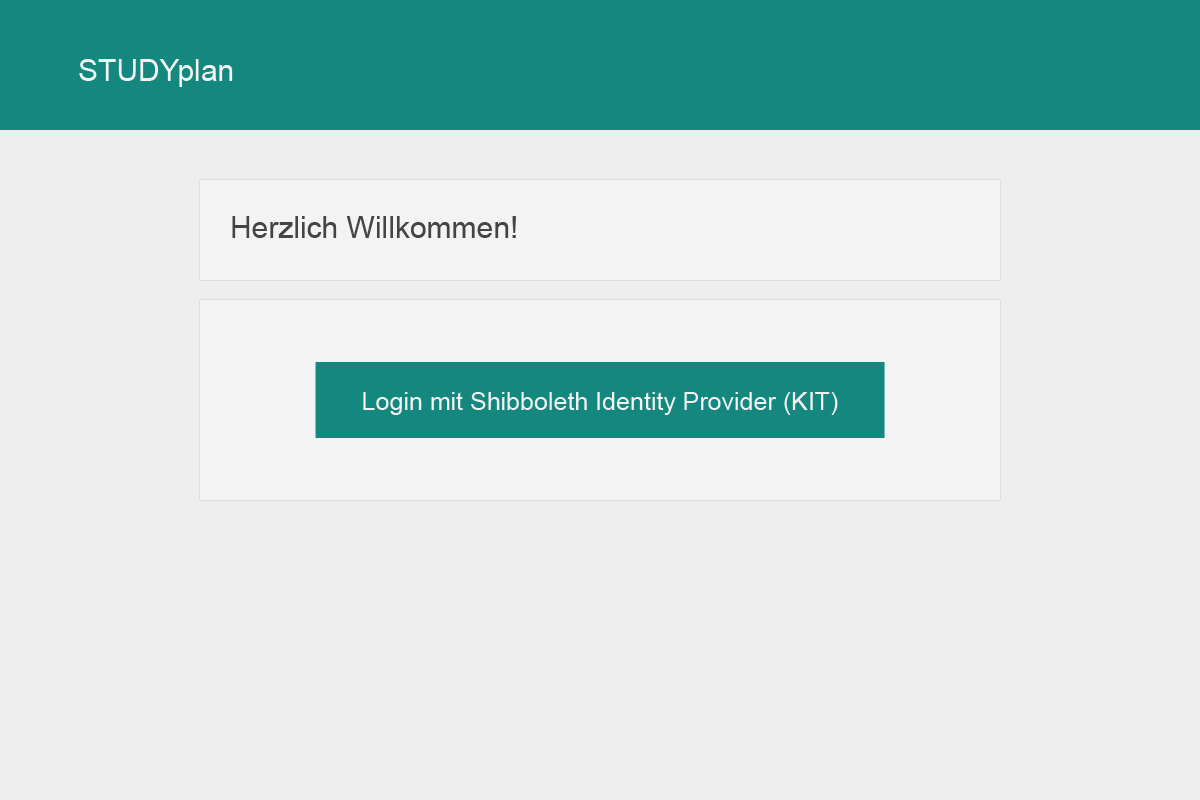
\includegraphics[width=0.8\textwidth]{../GUI/ergebnisse/login-1.png}
\end{figure}
\begin{figure}[!h]
	\caption{Erste Seite des Registrierungs"=\gls{Wizard}s mit Eingabe von Studienfach und Studienbeginn}
	\label{fig:gui-registrierung-1}
	\centering
	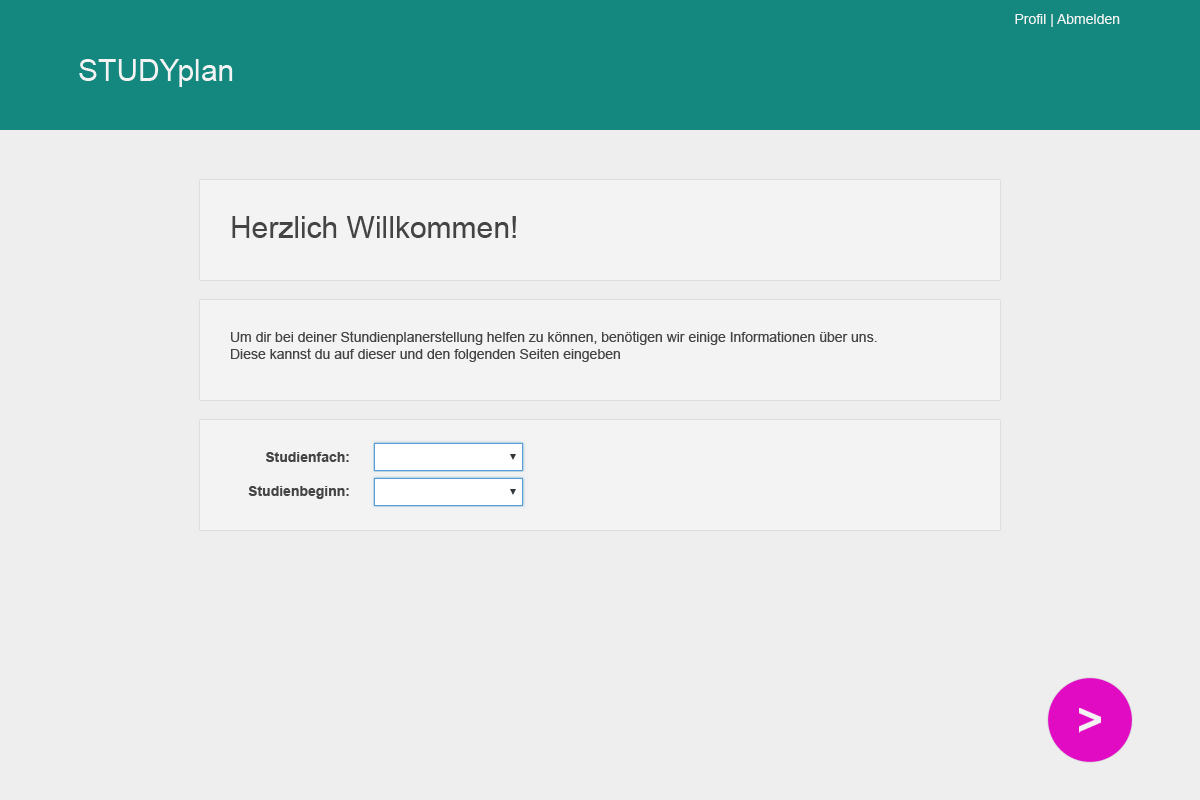
\includegraphics[width=0.8\textwidth]{../GUI/ergebnisse/registrierung-1.png}
\end{figure}

\begin{figure}
	\caption{Zweite Seite des Registrierungs"=\gls{Wizard}s mit Eingabe der schon begonnenen Module}
	\label{fig:gui-registrierung-2}
	\centering
	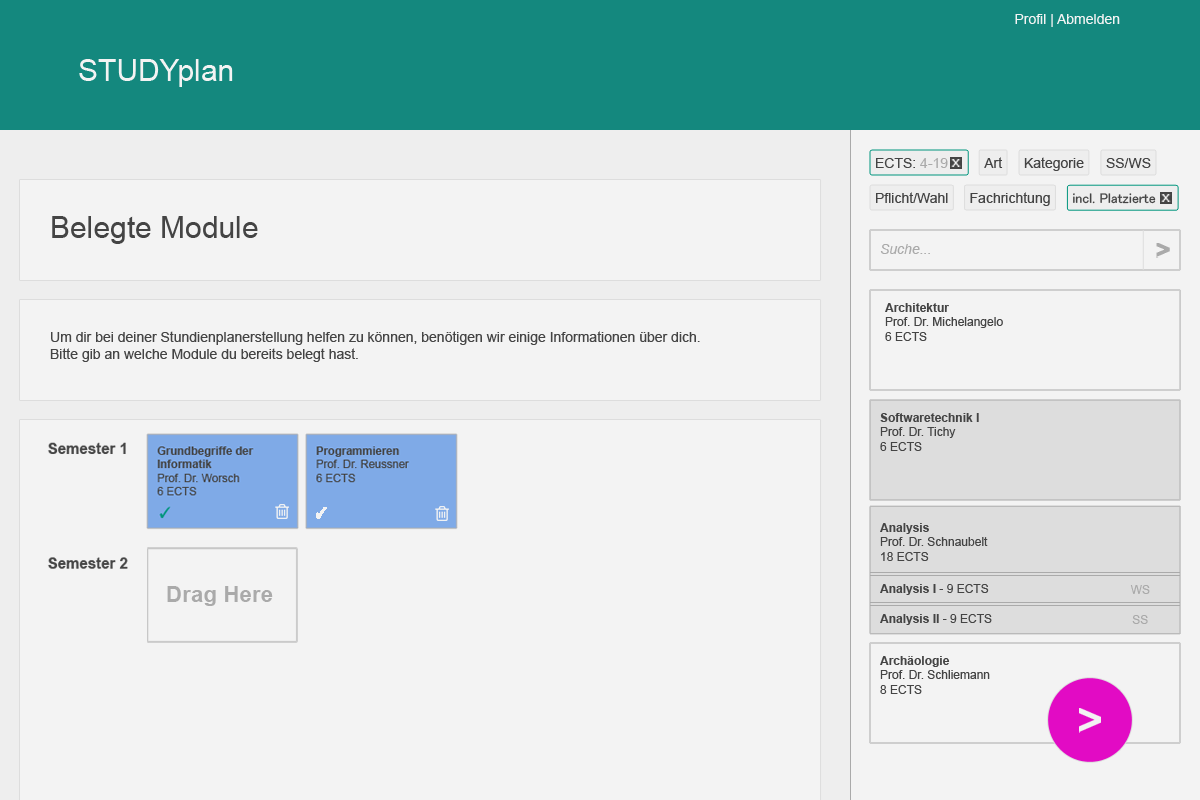
\includegraphics[width=0.9\textwidth]{../GUI/ergebnisse/registrierung-2.png}
\end{figure}

\begin{figure}
	\caption{Hauptseite des Systems}
	\label{fig:gui-hauptseite-1}
	\centering
	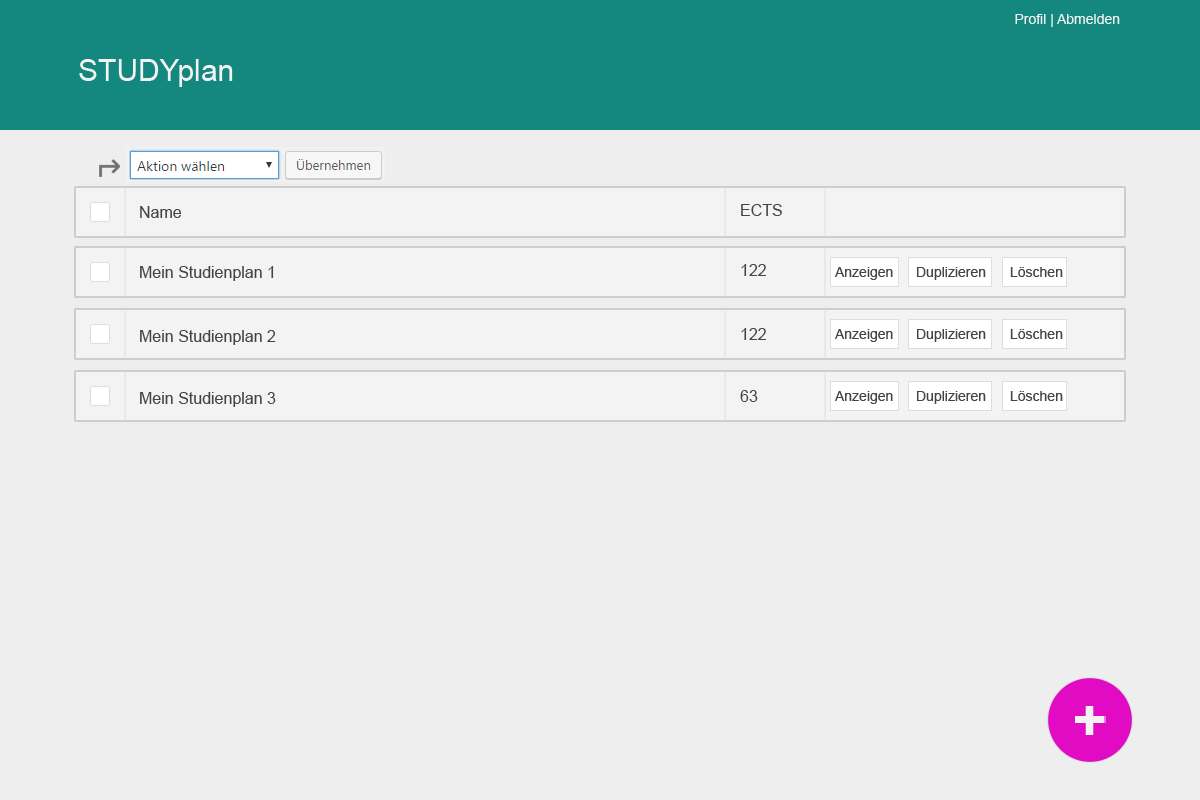
\includegraphics[width=0.9\textwidth]{../GUI/ergebnisse/hauptseite-1.png}
\end{figure}
\begin{figure}
	\caption{Manuelle Bearbeitung des Studienplans}
	\label{fig:gui-bearbeitung-1}
	\centering
	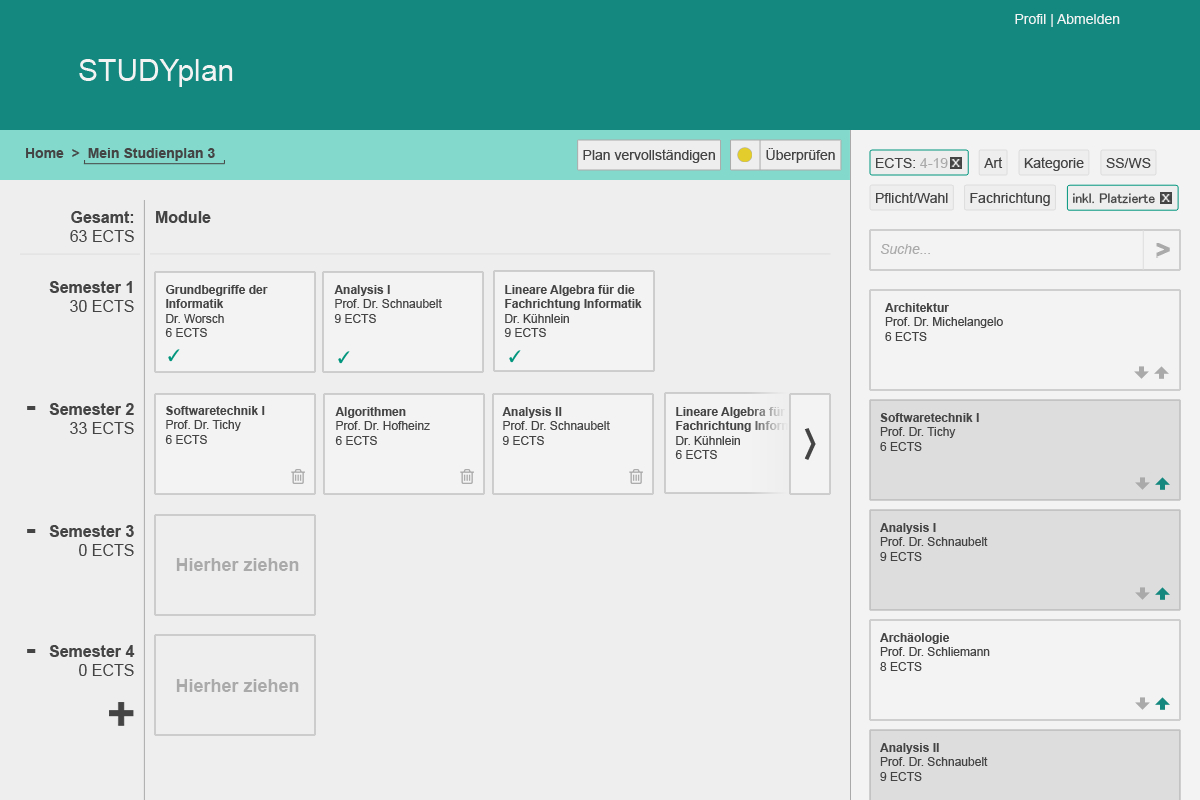
\includegraphics[width=0.9\textwidth]{../GUI/ergebnisse/bearbeitung-1.png}
\end{figure}
\begin{figure}
	\caption{Seitenleiste für Modulfilterung mit offener Kategorie-Auswahl}
	\label{fig:gui-module-filtern-1}
	\centering
	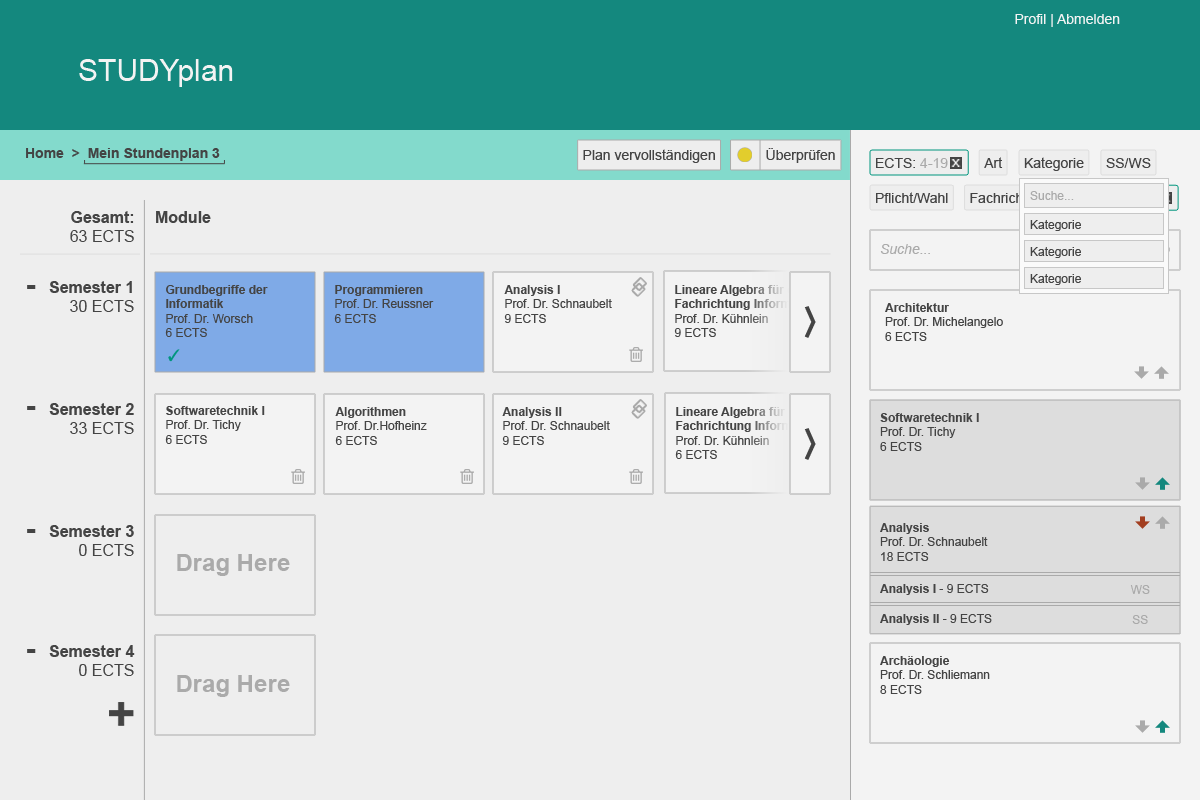
\includegraphics[width=0.9\textwidth]{../GUI/ergebnisse/module-filtern-1.png}
\end{figure}
\begin{figure}
	\caption{Seitenleiste für Modulfilterung mit offener ECTS-Auswahl}
	\label{fig:gui-module-filtern-2}
	\centering
	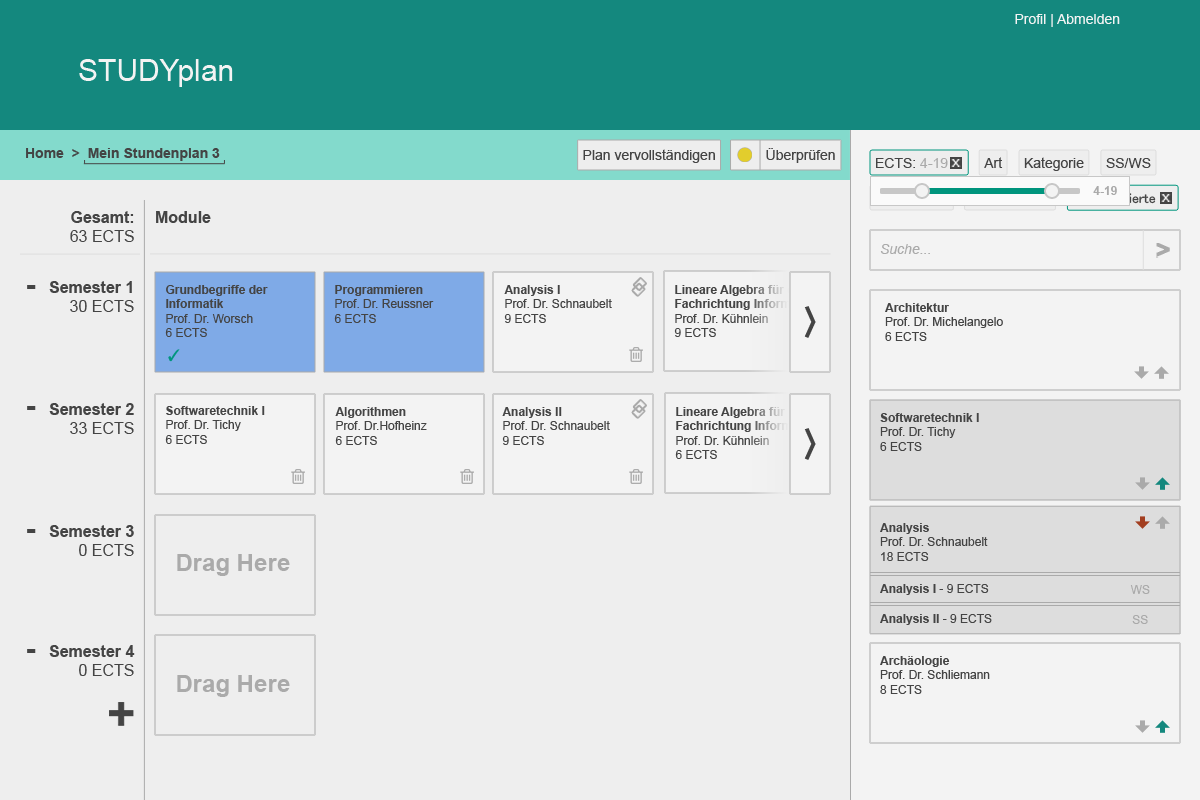
\includegraphics[width=0.9\textwidth]{../GUI/ergebnisse/module-filtern-2.png}
\end{figure}
\begin{figure}
	\caption{Detailansicht für Modul}
	\label{fig:gui-modul-info-1}
	\centering
	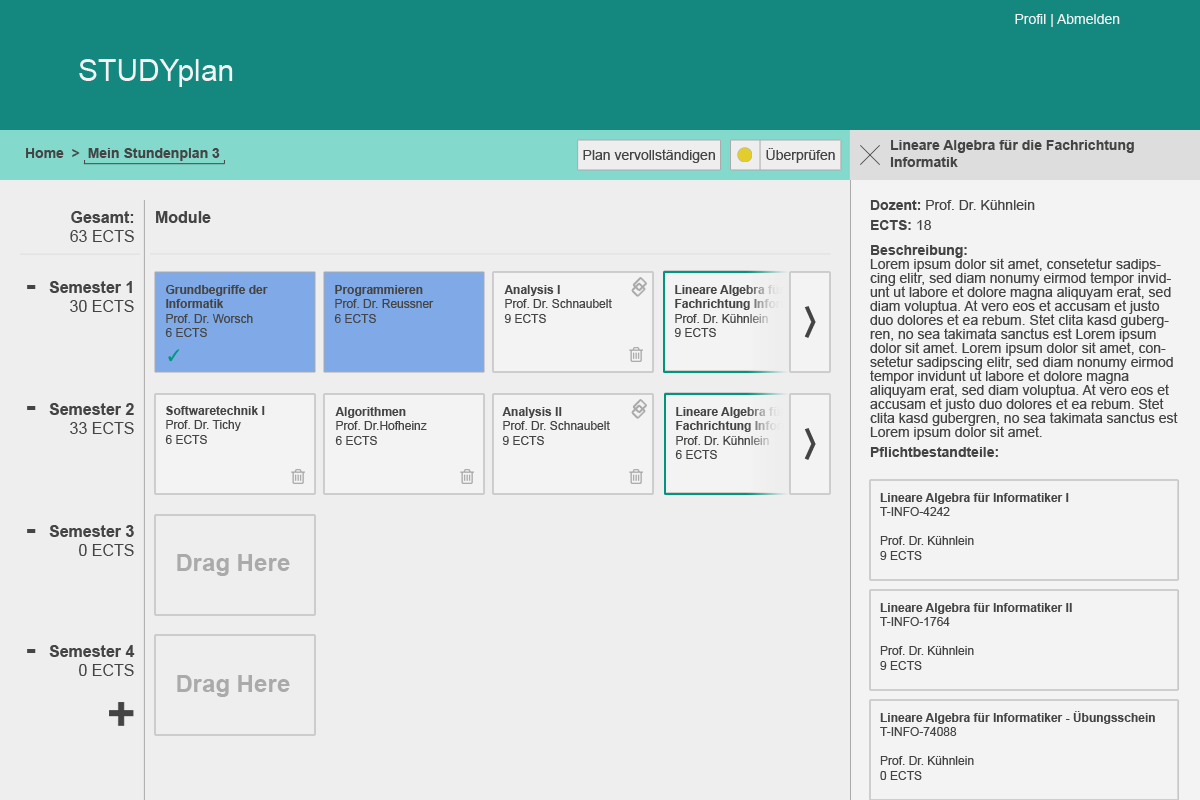
\includegraphics[width=0.9\textwidth]{../GUI/ergebnisse/modul-info-1.png}
\end{figure}
\begin{figure}
	\caption{1. Seite des Generierungs-Wizards}
	\label{fig:gui-generierung-1}
	\centering
	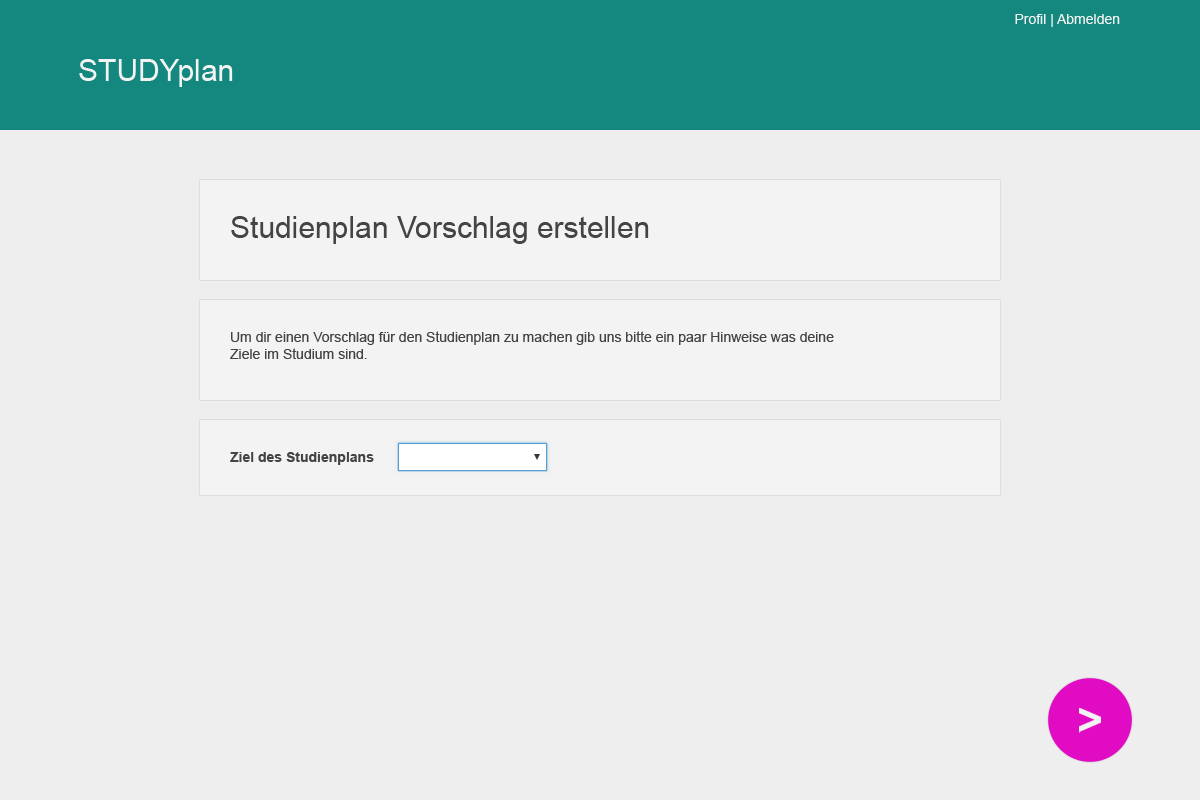
\includegraphics[width=0.9\textwidth]{../GUI/ergebnisse/generierung-1.png}
\end{figure}

\begin{figure}
	\caption{2. Seite des Generierungs-Wizard}
	\label{fig:gui-generierung-2}
	\centering
	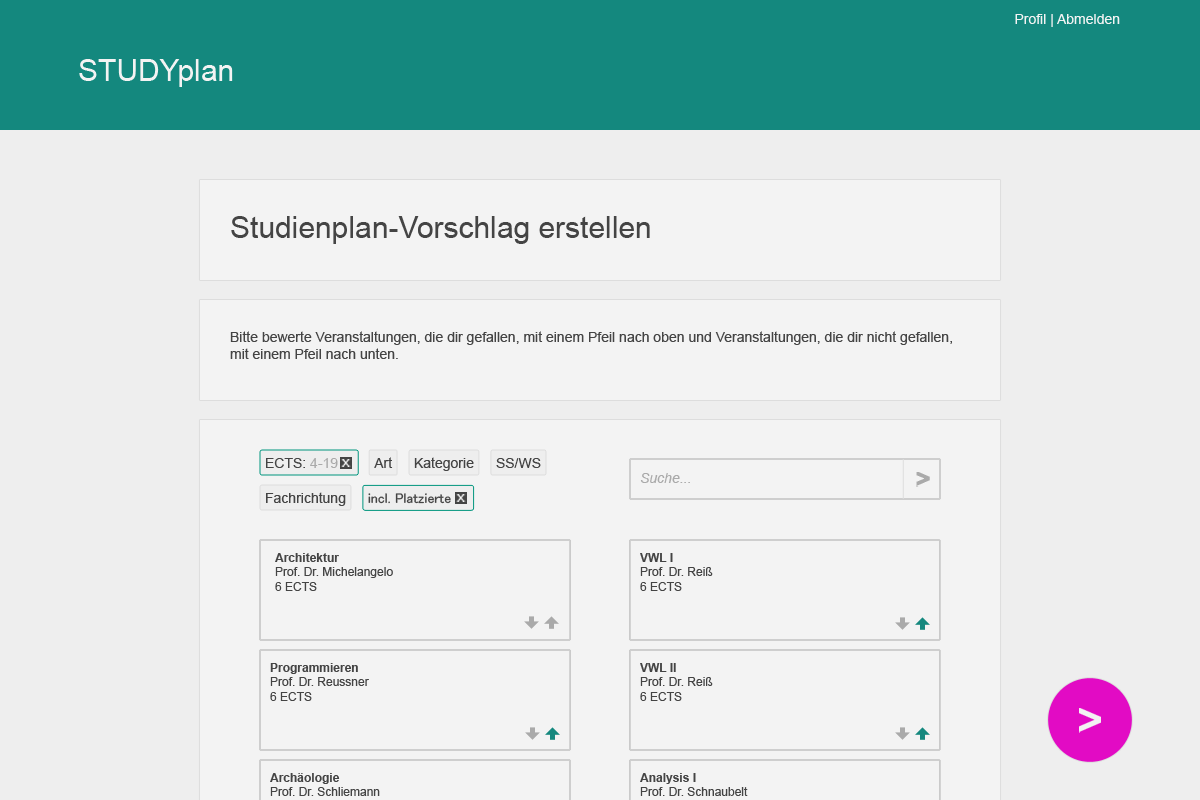
\includegraphics[width=0.9\textwidth]{../GUI/ergebnisse/generierung-2.png}
\end{figure}

\begin{figure}
	\caption{3. Seite des Generierungs-Wizard}
	\label{fig:gui-generierung-3}
	\centering
	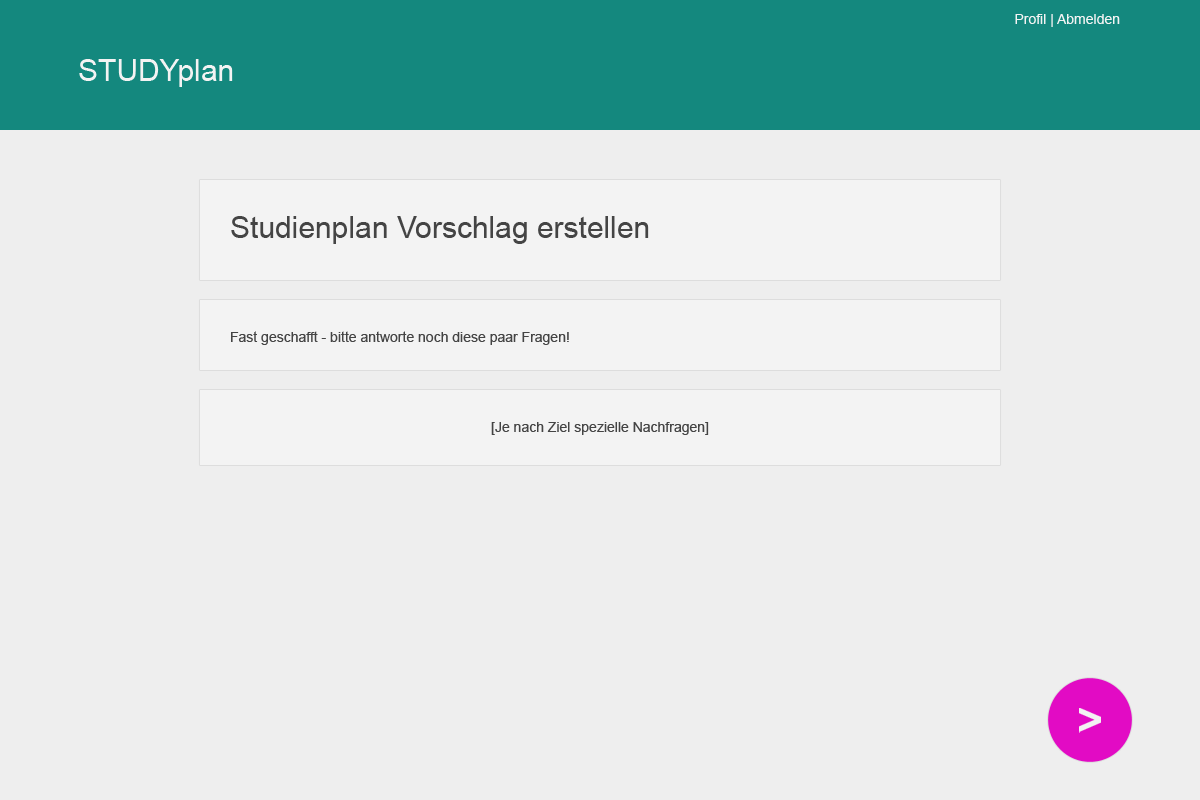
\includegraphics[width=0.9\textwidth]{../GUI/ergebnisse/generierung-3.png}
\end{figure}

\begin{figure}
	\caption{Anzeige des generierten Studienplans}
	\label{fig:gui-generierung-4}
	\centering
	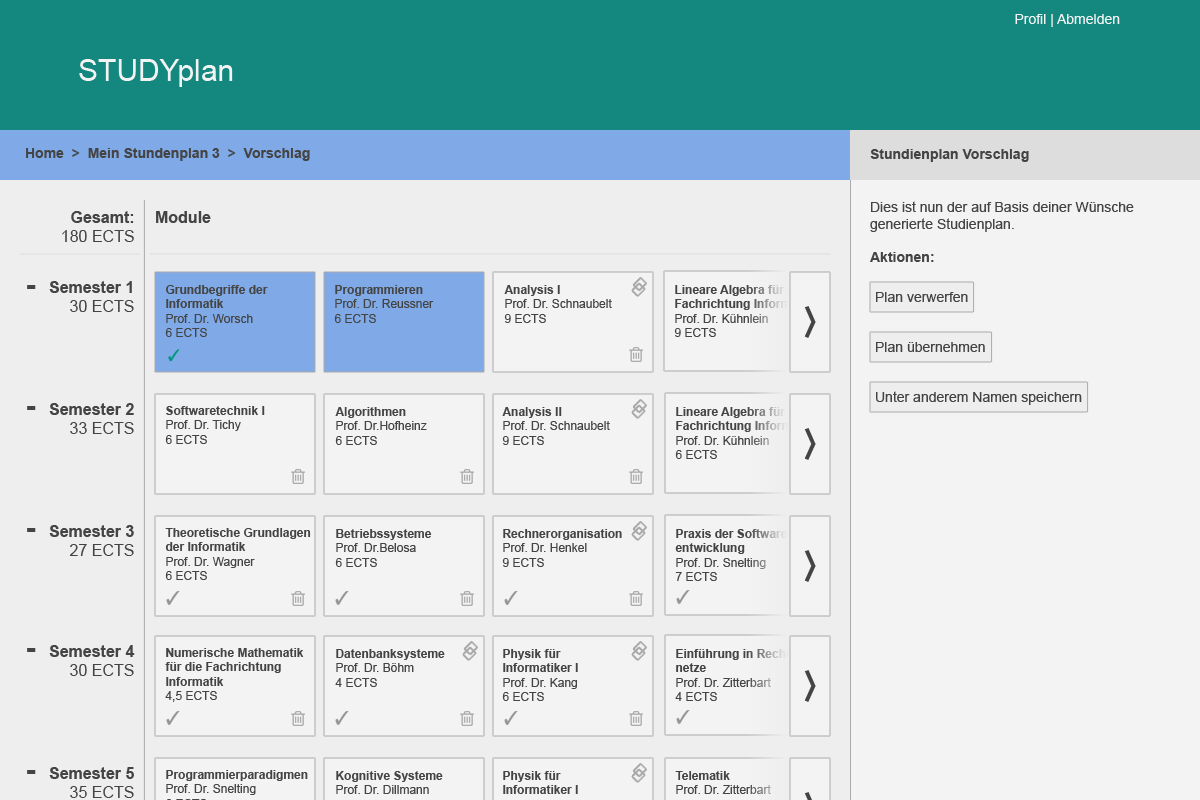
\includegraphics[width=0.9\textwidth]{../GUI/ergebnisse/generierung-4.png}
\end{figure}
\begin{figure}
	\caption{Erfolgreiche Verifizierung}
	\label{fig:gui-verifizierung-1}
	\centering
	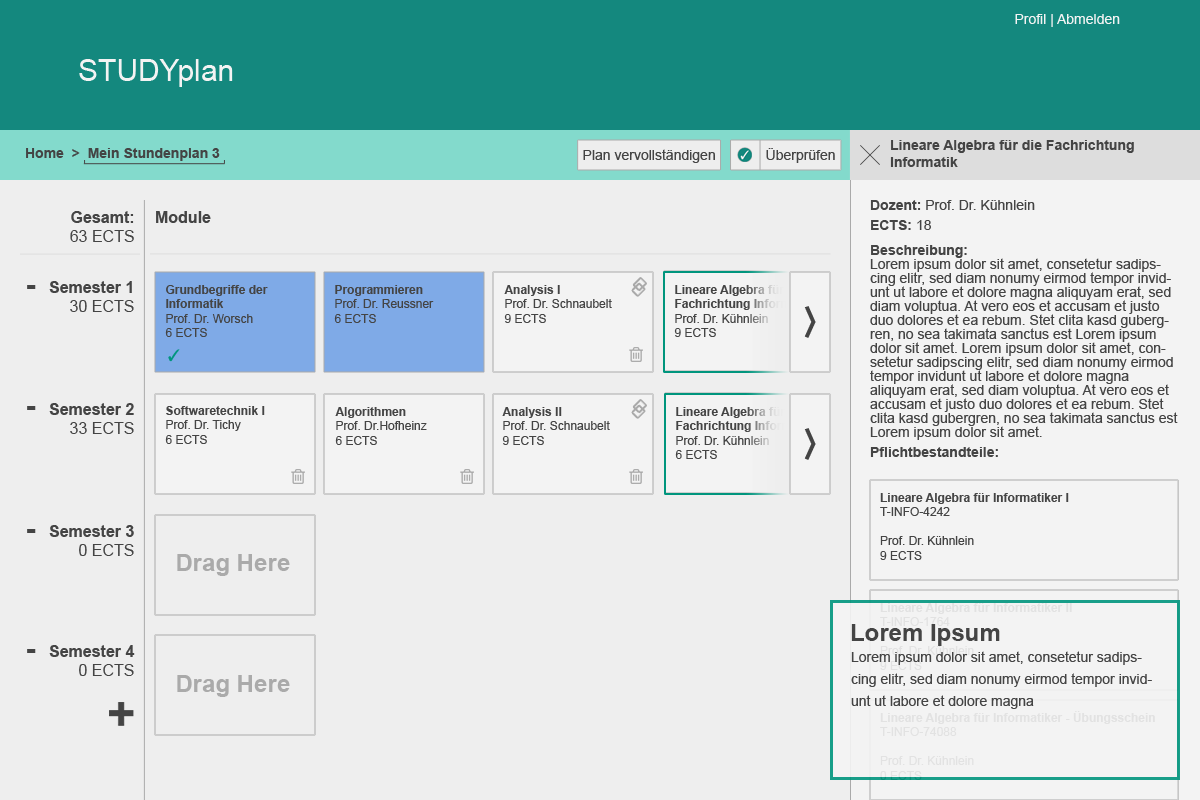
\includegraphics[width=0.9\textwidth]{../GUI/ergebnisse/verifizierung-1.png}
\end{figure}
\begin{figure}
	\caption{Fehlgeschlagene Verifizierung}
	\label{fig:gui-verifizierung-2}
	\centering
	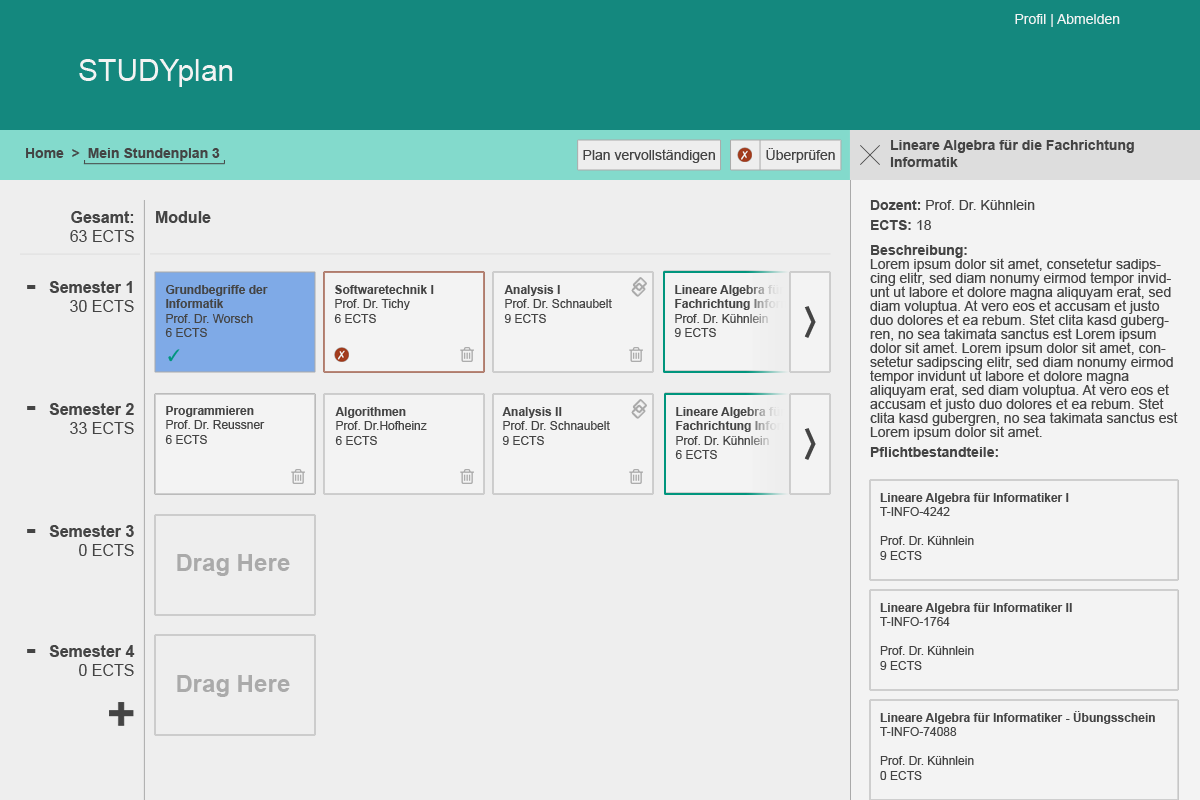
\includegraphics[width=0.9\textwidth]{../GUI/ergebnisse/verifizierung-2.png}
\end{figure}
\begin{figure}
	\caption{Profilansicht}
	\label{fig:gui-profil-1}
	\centering
	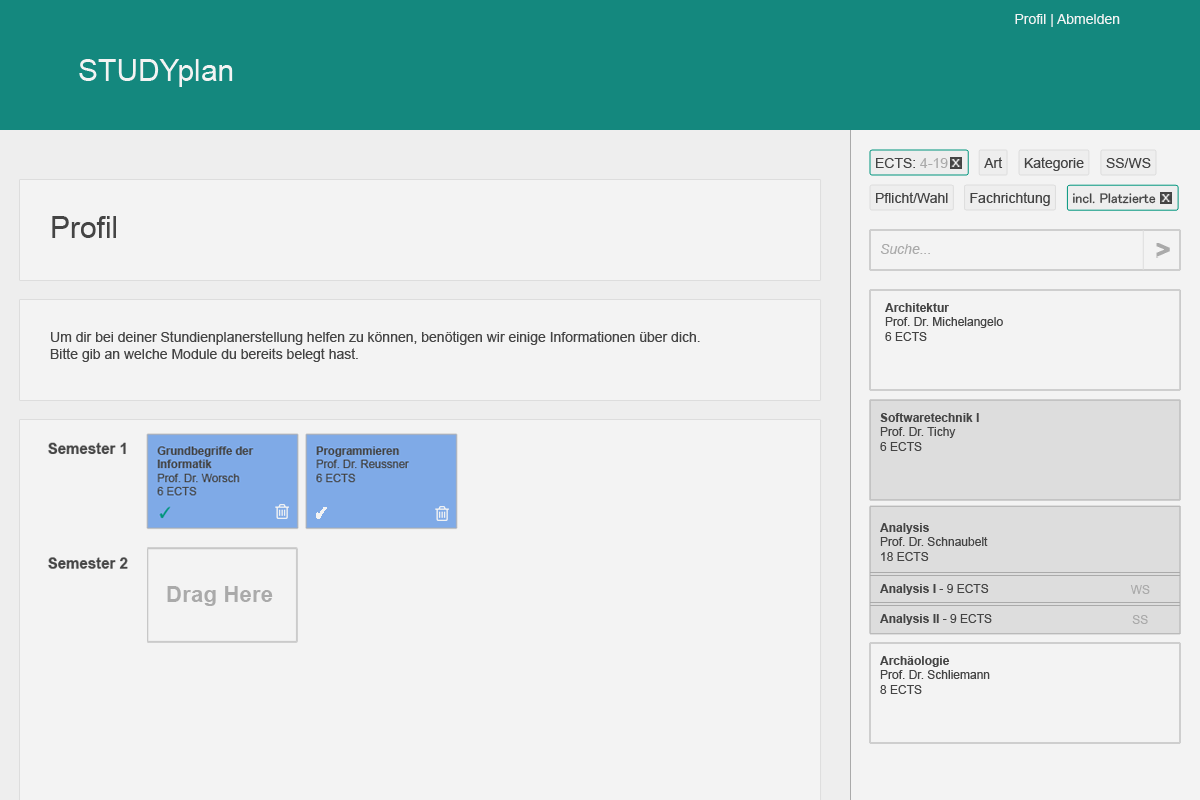
\includegraphics[width=0.9\textwidth]{../GUI/ergebnisse/profil-1.png}
\end{figure}
\FloatBarrier

	\printglossaries
	
	\begin{thebibliography}{9}
\bibliographystyle{plain}
\bibitem{rfc6749}
  D. Hart.
  \emph{The OAuth 2.0 Authorization Framework}.
  \url{https://tools.ietf.org/html/rfc6749}.
  IETF.
  2012.
 
\bibitem{rfc3986}
	T. Berners-Lee, R. Fielding and L. Masinter.
	\emph{Uniform Resource Identifier (URI): Generic Syntax}.
	\url{https://tools.ietf.org/html/rfc3986}.
	Network Working Group.
	2005.

\end{thebibliography}
\end{appendices}
\end{document}
